%%=============================================================================
%% Onderzoek
%%=============================================================================

\chapter{Testen}
\label{ch:testen}

In dit hoofdstuk zullen de uitgevoerde experimenten en testen uiteengezet en besproken worden, volgens de richtlijnen aangehaald in Hoofdstuk~\ref{ch:methodologie}. Ze zullen gesorteerd staan volgens opstelling en gerangschikt in dezelfde volgorde als in Hoofdstuk~\ref{ch:opstellingen}.

\section{RFID}
Voor elk van volgende testen bestaat data over zowel de RSSI als het relatieve faseverschil. Het verloop van het relatieve faseverschil is gelijkaardig aan de RSSI, aangezien beide afhankelijk zijn van de afstand tussen de antenne en de tag. Alhoewel de grafieken van het relatieve faseverschil veelal een mooier verloop hebben, is er gekozen de conclusies van volgende testen te nemen op basis van de RSSI grafieken, dit aangezien de relatieve fase een berekende waarde is, berekend uit het absolute faseverschil. Deze berekening is echter niet in alle gevallen volledig correct, waardoor er onvoorziene fenomenen zouden kunnen optreden in algoritmes gebaseerd op deze data. Echter is het in theorie mogelijk dezelfde conclusies te bekomen gebaseerd op (correcte) absolute fasedata.
Verder is er bij alle statische testen data over de in en de uit richting van de locatie, hiervan zal slechts 1 worden getoond aangezien beide richtingen dezelfde info verschaffen, dit uiteraard tenzij beide tonen een meerwaarde geeft.
Alle volgende grafieken zijn gegenereerd door ARTA, waarin het helaas niet mogelijk is om een asbenaming te doen. In alle RSSI grafieken vertegenwoordigd de x-as te tijd (in seconden) en de y-as de RSSI waarde (in dBm).

\subsection{1 antenne aan deurlijst}
\subsubsection{Deelhypothese}
Deze opstelling kan het voorbijkomen van een getagd asset waarnemen.

\subsubsection{Test: PoC}
Deze eerste en enige test voor deze opstelling is een Proof of concept test. Hier zal worden nagegaan of en hoe een voorbijkomende tag zal geregistreerd worden. Voor de opstelling is 1 antenne gebruikt die vlak aan een deurkader is gehangen, en de tag zal op een afstand van ~30 cm voorbij komen door het deurgat, dit in een horizontale positie in een evenwijdig vlak aan de antenne.

\begin{minipage}{0.55\textwidth}
In bijhorende grafiek is zichtbaar dat een voorbijkomende tag wordt geregistreerd door de reader met een piek in de RSSI waarde.
\end{minipage}
\hfill
\begin{minipage}{0.42\textwidth}
	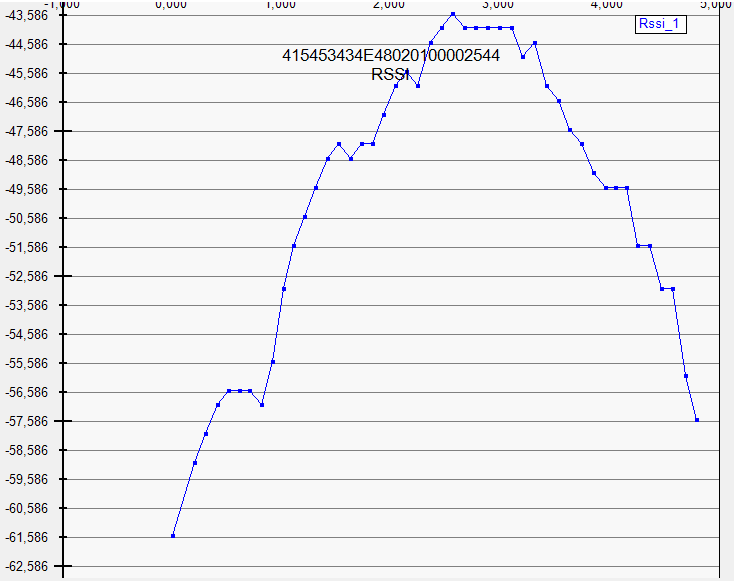
\includegraphics[width=\linewidth]{0_RSSI}
\end{minipage}

\subsubsection{Deelconclusie}
Uit deze test is duidelijk dat een voorbijkomende tag, bij uitbreiding een getagd asset die de locatie binnenkomt, correct geregistreerd zal worden door het systeem. De hypothese is dus bevestigd. Buiten deze simpele registratietest is er ook nood aan het testen van de invloed van tag oriëntatie en afstand tegenover de antenne. Deze fenomenen worden echter ook onderzocht in de volgende opstelling en zijn hier dus niet apart onderzocht. De beschouwingen en conclusies van test 1 en 2 in de opstelling met 2 antennes zijn dus ook toepasselijk op deze opstelling, uiteraard vereenvoudigd naar 1 antenne.

\subsection{2 antennes aan deurlijst}
\subsubsection{Deelhypothese}
Deze opstelling kan het voorbijkomen en de richting van een getagd asset waarnemen, genomen dat de afstand tussen de tag en de antenne voldoende klein is.

\subsubsection{Test 1: Oriëntatie van de tag}
In deze eerste test wordt de invloed van de oriëntatie van de tag tegenover de antennes bepaald, aangezien deze oriëntatie in theorie een invloed heeft op de gemeten RSSI waarde. De opstelling voor deze test is als volgt: 2 antennes zijn in een deuropening geplaatst, naast elkaar. Bij het binnenkomen wordt eerst antenne 1, en daarna antenne 2 gepasseerd. Er worden 4 oriëntaties onderzocht, nl. horizontaal (a) en verticaal (b) in een evenwijdig vlak aan de antennes, en horizontaal (c) en verticaal (d) loodrecht op het vlak van de antennes. Voor elk van deze deeltesten geld een afstand tussen de tag en de antenne van ~30cm. Bij elk scenario is zowel de richting in als uit getest, echter zullen deze resultaten enkel beide worden getoond als er een meerwaarde is.
In theorie zouden a en b ruwweg dezelfde resultaten moeten geven, terwijl c en d een lagere RSSI zouden moeten geven. Echter zou het in elk geval detecteerbaar moeten zijn.

\paragraph{a) Horizontaal in antennevlak}
\begin{minipage}{0.55\textwidth}
Uit bijhorende grafiek, die de tag toont die uit de locatie ging, is duidelijk een opeenvolging van pieken te zien. Dit met volgorde 2 (groen) -> 1 (blauw), wat inderdaad uit de locatie gaan is. Deze detectie is dus geslaagd. De piekhoogte is niet gelijk, ondanks dat de antennes hetzelfde type zijn. Dit is kalibreerbaar maar zoals zichtbaar is dit niet nodig voor een toepassing als deze.
\end{minipage}
\hfill
\begin{minipage}{0.42\textwidth}
	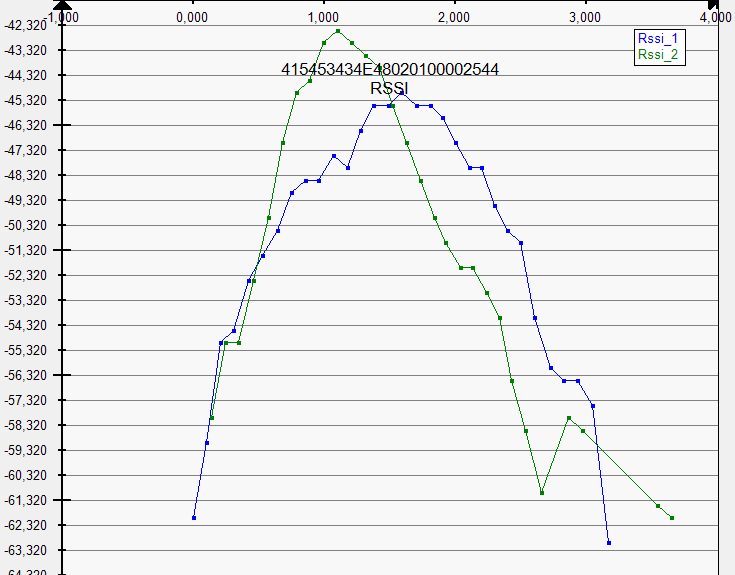
\includegraphics[width=\linewidth]{1a_uit_RSSI}
\end{minipage}

\paragraph{b) Verticaal in antennevlak}
\begin{minipage}{0.55\textwidth}
In deze grafiek is vrij gelijkaardig aan de vorige, wat theoretisch ook zou moeten. Er zijn duidelijk 2 pieken zichtbaar, in de juiste volgorde volgend de tag die uit de locatie gaat. Ook is de RSSI gelijkaardig (rond de -40 à -45 dBm).
\end{minipage}
\hfill
\begin{minipage}{0.42\textwidth}
	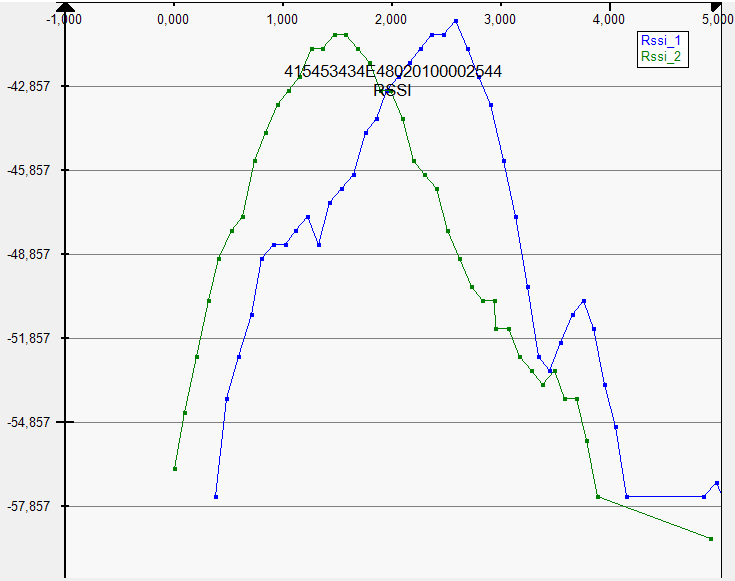
\includegraphics[width=\linewidth]{1b_uit_RSSI}
\end{minipage}

\paragraph{c) Horizontaal loodrecht op antennevlak}
\begin{minipage}{0.55\textwidth}
In deze grafiek is een beweging van de tag naar in de locatie weergegeven, hoewel de toppen duidelijk zichtbaar zijn, en in de correcte richting staan, is de top minder duidelijk afgelijnd en meer uitgerokken. Ditzelfde fenomeen is ook zichtbaar in de uit-richting. Ook liggen de toppen iets lager dan de toppen in de vorige 2 deeltests.
\end{minipage}
\hfill
\begin{minipage}{0.42\textwidth}
	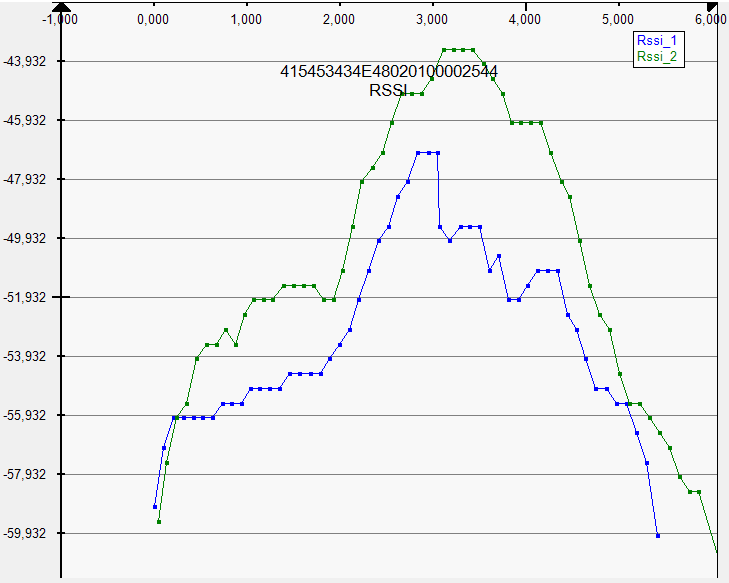
\includegraphics[width=\linewidth]{1c_in_RSSI}
\end{minipage}

\paragraph{d) Verticaal loodrecht op antennevlak}
\begin{minipage}{0.55\textwidth}
In deze grafiek in ook een beweging van de tag naar in de locatie weergegeven, en is het fenomeen van meer uitgerokken toppen nog beter zichtbaar. De uit richting vertoont wederom hetzelfde patroon. Deze deeltest ligt dus in lijn met de vorige, maar nog opvallender.
\end{minipage}
\hfill
\begin{minipage}{0.42\textwidth}
	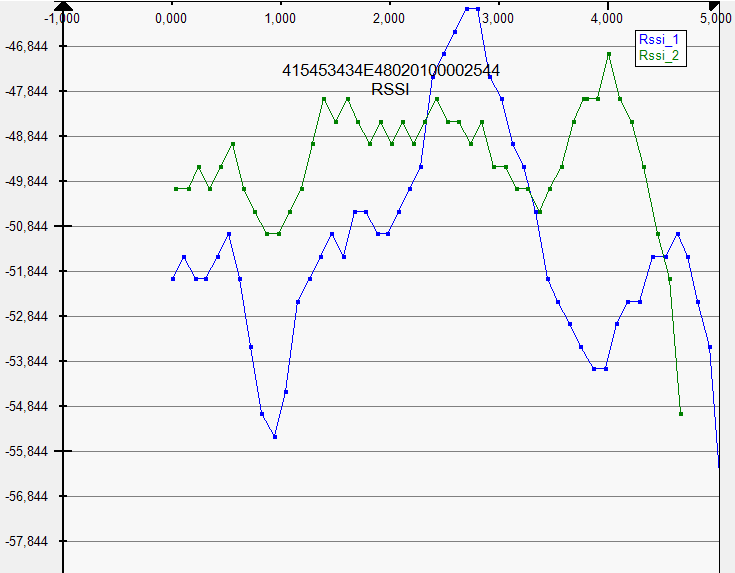
\includegraphics[width=\linewidth]{1d_in_RSSI}
\end{minipage}

\paragraph{Testconclusie}
Zoals verwacht is de detectie van de tag en de richting ervan goed zichtbaar en in elk geval correct gemeten. Ook is de meetkwaliteit minder als de tags niet in het vlak van de antenne liggen, daarom lijkt het aanbevolen dit zo veel mogelijk te vermijden.

\subsubsection{Test 2: Afstand tussen tag en antennes}
In deze test wordt de invloed van de afstand tussen de tag en de antennes gemeten, in theorie zou de RSSI van de piek lager moeten zijn als de tag verder van de antenne voorbij komt, en door de conische vorm van het meetveld van de vlakke antenne zouden de pieken meer moeten overlappen. De testopstelling is idem aan Test 1, de oriëntatie van de tag is constant gehouden op horizontaal in hetzelfde vlak als de antennes, en de richting is uit de locatie. De gemeten afstanden zijn 5cm afstand (zeer dicht) en 100cm afstand (zeer ver). Dit kan vergeleken worden met de resultaten van Test 1a, aangezien dit dezelfde opstelling betreft, op 30 cm afstand.

\paragraph{a) 5cm}
\begin{minipage}{0.55\textwidth}
Op deze grafiek is het verwachte resultaat te zien, 2 duidelijke pieken die licht verder uit elkaar liggen, en een hogere RSSI waarde hebben.
\end{minipage}
\hfill
\begin{minipage}{0.42\textwidth}
	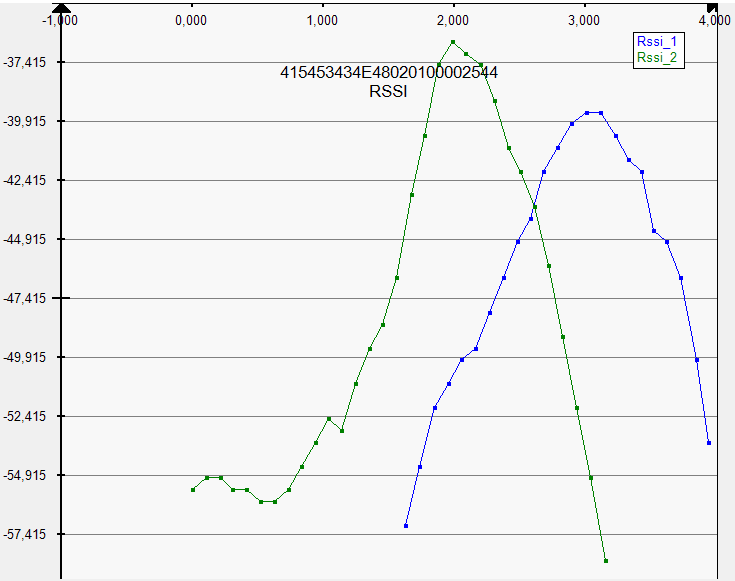
\includegraphics[width=\linewidth]{2a_RSSI}
\end{minipage}

\paragraph{b) 100cm}
\begin{minipage}{0.55\textwidth}
Deze grafiek is interessanter dan de vorige, het vermoeden dat de piek minder duidelijk ging zijn en ging overlappen is bevestigd. Uit deze meting kan niet meer afgeleid worden in welke richting de tag voorbij de antennes komt. Ook ligt de RSSI waarde beduidend lager.
\end{minipage}
\hfill
\begin{minipage}{0.42\textwidth}
	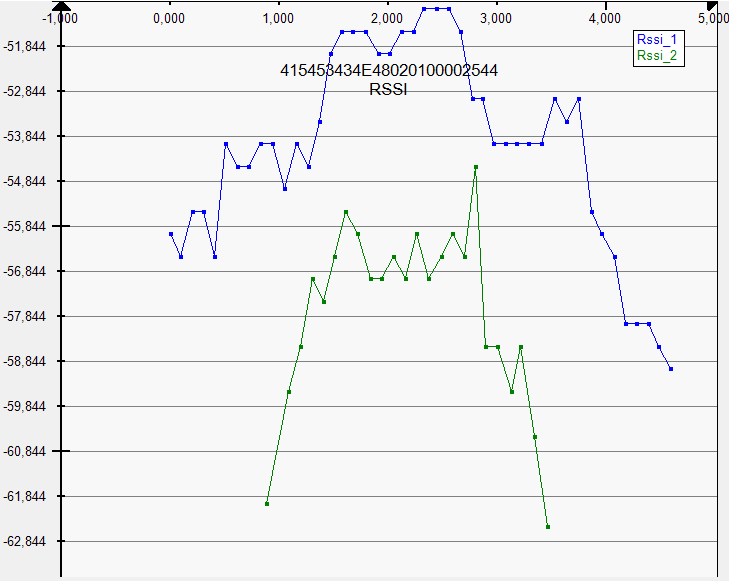
\includegraphics[width=\linewidth]{2b_RSSI}
\end{minipage}

\paragraph{Testconclusie}
Zoals werd vermoed is er een bepaalde restrictie op de afstand waarmee de tag de antennes kan voorbijkomen om een goede richtingsdetectie te hebben. 

\subsubsection{Test 3: Afstand tussen de 2 antennes}
Aangezien de reden van de overlappende pieken in vorige test het feit is dat het conische bereik van de 2 antennes elkaar te veel overlapt, is het logisch dat dit effect zal verminderen als deze 2 antennes verder van elkaar geplaatst worden, dit zal getest worden in deze 3e test. De opstelling is identiek aan de test 2, het enige verschil is dat de 2 antennes 20cm uit elkaar gezet zijn.

\paragraph{a) 5cm}
\begin{minipage}{0.55\textwidth}
Dit testresultaat toont wederom 2 mooie pieken, deze keer iets verder uit elkaar liggend door de afstand tussen de antennes, en dit met een lage RSSI waarde.
\end{minipage}
\hfill
\begin{minipage}{0.42\textwidth}
	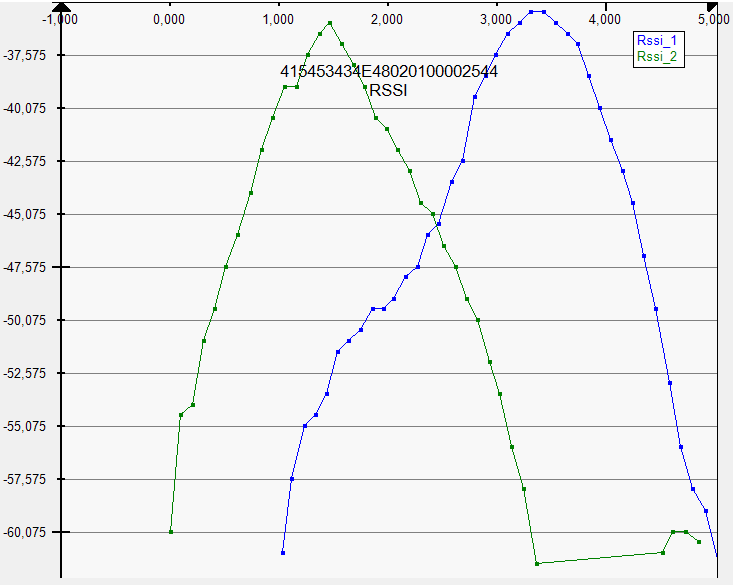
\includegraphics[width=\linewidth]{3a_RSSI}
\end{minipage}

\paragraph{b) 30cm}
\begin{minipage}{0.55\textwidth}
Hier zien we ongeveer hetzelfde als op de vorige grafiek, enkel licht meer uitgerokken en met een lagere RSSI waarde.
\end{minipage}
\hfill
\begin{minipage}{0.42\textwidth}
	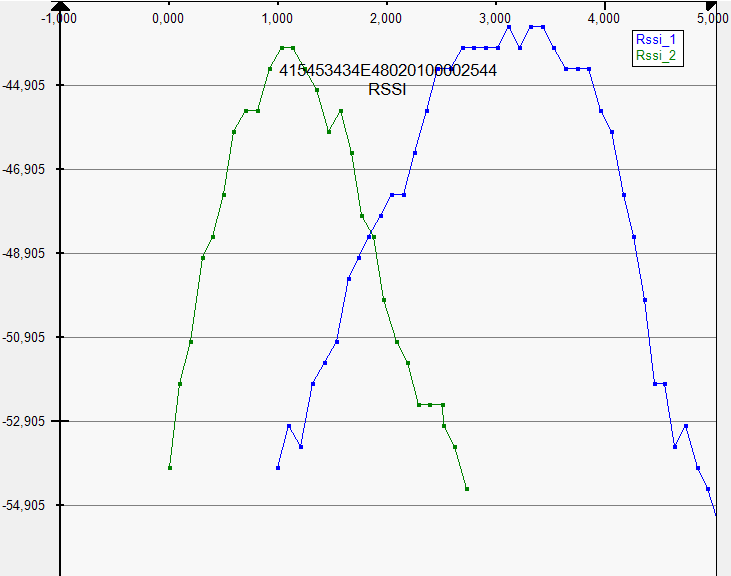
\includegraphics[width=\linewidth]{3b_RSSI}
\end{minipage}

\paragraph{b) 100cm}
\begin{minipage}{0.55\textwidth}
Dit resultaat is het voornaamste van deze test, we zien, zoals bij test 2, dat de pieken weer hard zijn uitgerokken, maar door de extra afstand tussen de antennes is de volgorde wel weer zichtbaar.
\end{minipage}
\hfill
\begin{minipage}{0.42\textwidth}
	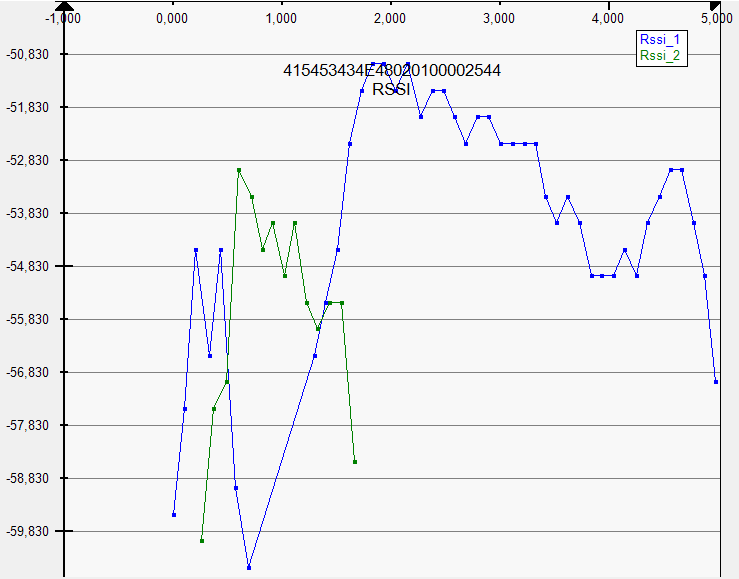
\includegraphics[width=\linewidth]{3c_RSSI}
\end{minipage}

\paragraph{Testconclusie}
Het blijkt inderdaad correct dat het verder uit elkaar plaatsen van de antennes een positief effect heeft op het uit elkaar trekken van de pieken in de RSSI curve, wat nodig is naarmate de tag verder van de antenne voorbij komt.

\subsubsection{Deelconclusie}
Deze opstelling slaagt er inderdaad in om een voorbijkomende tag en zijn richting te registreren, mits de afstand beperkt is, de hypothese is dus correct. Er kan echter wel aan toegevoegd worden dat, als de afstand niet meer voldoende klein is, dat de afstand tussen de antennes kan vergroot worden. Dit is in een reële situatie echter niet praktisch aangezien een deur meestal een beperkte breedte heeft. Voor een standaard deur zal dit geen probleem zijn aangezien de maximale afstand in een deur ook beperkt is, maar voor bv. een poortdoorgang kan dit wel problemen opleveren. In een gang met een quasi onbeperkte beschikbare breedte is dit wel mogelijk.

\subsection{1 antenne tegenover deur}
\subsubsection{Deelhypothese}
Deze opstelling kan het voorbijkomen en de richting van een getagd asset waarnemen, genomen dat de afstand tussen de antenne en de deur voldoende klein is zodat de antenne de tag kan registreren.

\subsubsection{Test 1: PoC}
Deze eerste test bestaat uit een proof of concept, hierin wordt getest of het op zijn minst mogelijk is om de richting van de bewegende tag te bepalen uit de gemeten data. 
In deze test wordt een antenne geplaatst tegen een muur, met daarvoor een kar met een tag op (horizontaal in het vlak van de antenne). Deze kar zal voor deze test achteruit en vooruit gerold worden. 

\paragraph{Resultaat}
Onderstaande grafieken tonen de verandering in RSSI van beide testen, met het rollen van de kar weg van de antenne links, en naar de antenne toe rechts. In deze grafieken is deze richting zeer mooi zichtbaar, de RSSI verlaagt als de kar wegrolt, en verhoogt als deze naar de antenne toe rolt.

\begin{minipage}{0.42\textwidth}
	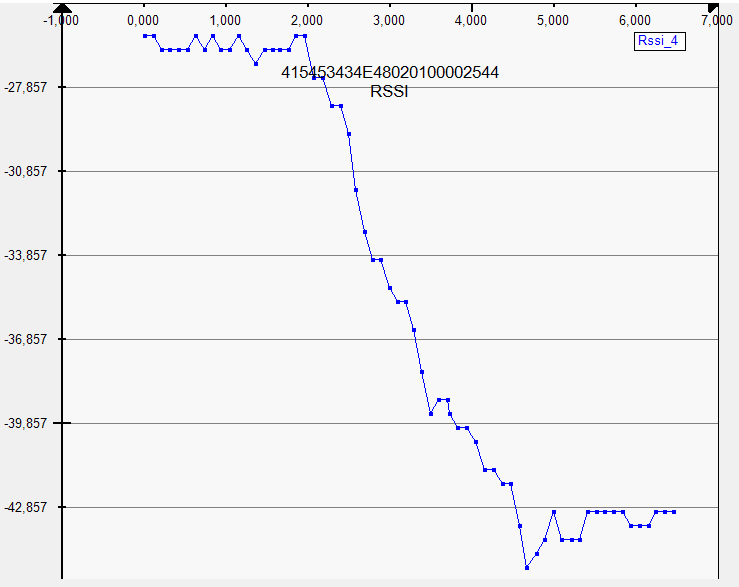
\includegraphics[width=\linewidth]{4c_RSSI}
\end{minipage}
\hfill
\begin{minipage}{0.42\textwidth}
	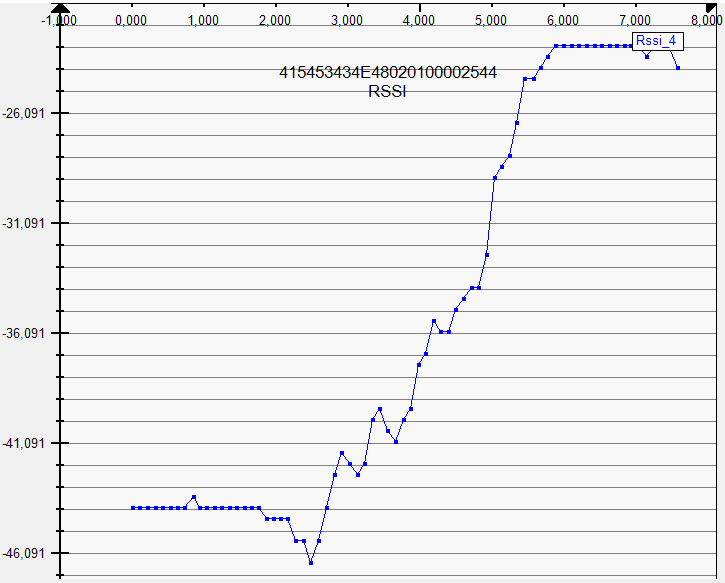
\includegraphics[width=\linewidth]{4d_RSSI}
\end{minipage}

\paragraph{Testconclusie}
Uit deze resultaten is zeer mooi te zien dat de richting van de verplaatsing op de lijn voor een antenne duidelijk zichtbaar is.

\subsubsection{Test 2: Variabele afstand tot deur}
In deze test wordt de opstelling realistischer gemaakt, de antenne wordt op respectievelijk 100 en 200 cm afstand van de deur geplaatst, en er wordt met de kar met bevestigde RFID tag van test 1 door de deur gereden, zowel in als uit de kamer, direct de hoek om. 

\paragraph{a) 100cm}
Hieronder is het binnenkomen (links) en het verlaten (rechts) van de locatie te zien, zoals duidelijk te zien is is de grafiek zeer veel minder duidelijk dan in de ideale situatie van test 1. Vermoedelijk is de 'staart' die niet in de meting past (rechts aanhangsel bij inwaarts en links bij uitwaarts) het gevolg van het feit dat de kar op dat moment 90° gedraaid in de kamer aanwezig is, resp. na en voor de draaibeweging door de deur. Op dit moment bevind de tag zich in het leesveld van de antenne, maar niet meer in hetzelfde vlak. Deze onderlinge oriëntatie zorgt voor een slechte RSSI waarde, zoals aangetoond tijdens test 1 van de vorige opstelling. Voor de duidelijkheid van de 'uit' meting is dit niet zo zeer een probleem, maar wel voor de 'in' meting.

\begin{minipage}{0.42\textwidth}
	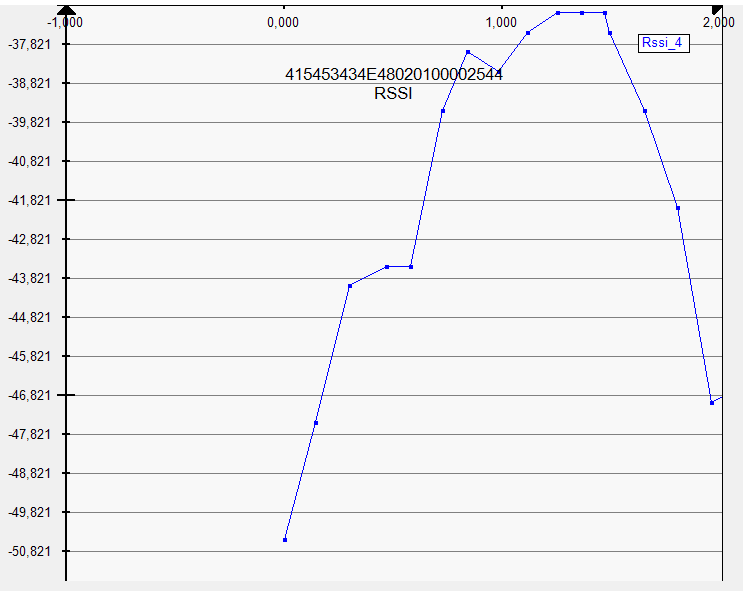
\includegraphics[width=\linewidth]{5a_in_RSSI}
\end{minipage}
\hfill
\begin{minipage}{0.42\textwidth}
	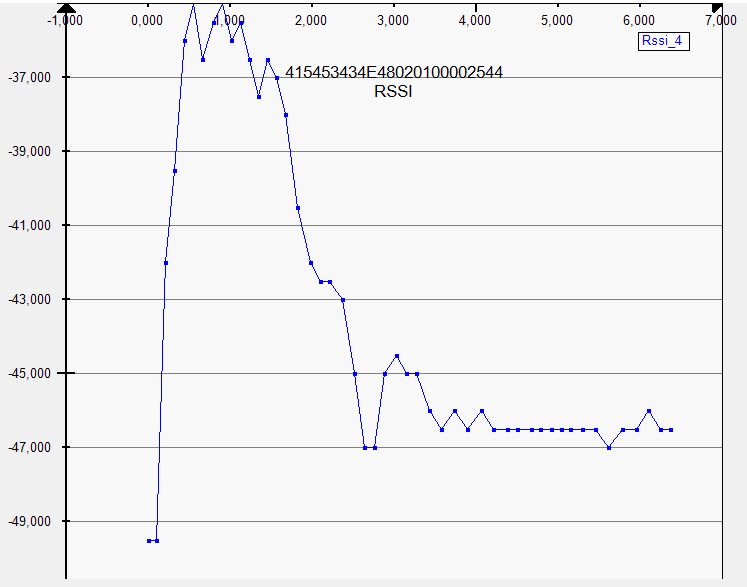
\includegraphics[width=\linewidth]{5a_uit_RSSI}
\end{minipage}

\paragraph{b) 200cm}
Hieronder is wederom het binnenkomen (links) en het verlaten (rechts) van de locatie te zien. In dit geval is de onduidelijkheid zichtbaar in vorige deeltest nog extremer zichtbaar. Alhoewel het in theorie de richting nog steeds eenduidig zichtbaar is, is het nog minder duidelijk, en deze onduidelijkheid vergroot naarmate de tussenliggende afstand groter wordt. Ook de RSSI waarde ligt logischerwijs lager.

\begin{minipage}{0.42\textwidth}
	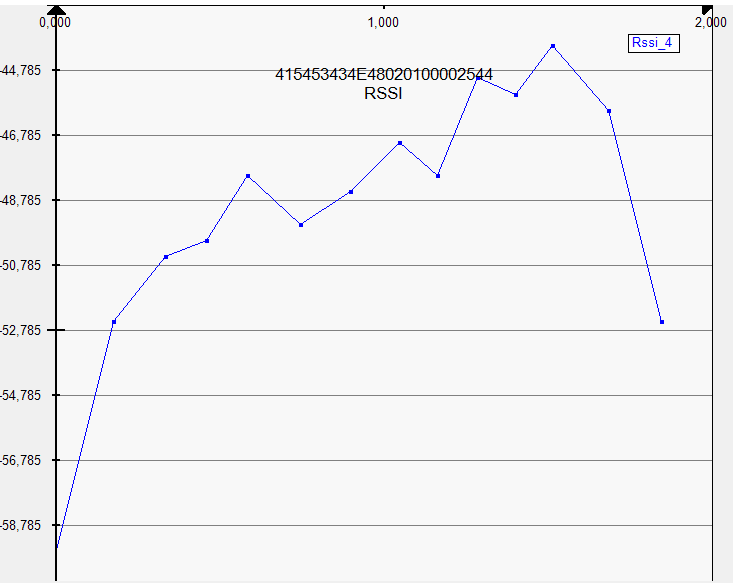
\includegraphics[width=\linewidth]{5b_in_RSSI}
\end{minipage}
\hfill
\begin{minipage}{0.42\textwidth}
	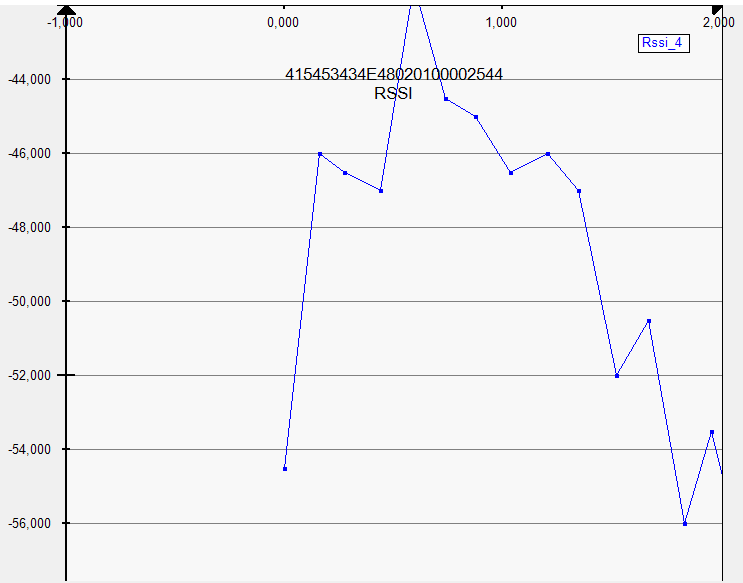
\includegraphics[width=\linewidth]{5b_uit_RSSI}
\end{minipage}

\paragraph{Testconclusie}
Deze testen tonen aan dat de meting in een realistisch scenario veel minder optimaal is als in het optimaal scenario van test 1 aangezien de meetpunten rond het dichter/verder komen voor onduidelijkheden zorgen die niet eenduidig uit de data te halen zijn.

\subsubsection{Test 3: Langere meetafstand}
Aangezien een simpele draai rond het deurgat te slechte data oplevert om eenduidig de richting te bepalen, kan het een idee zijn om de kar langer op de lijn van de antenne te laten rijden om zo het relatieve aantal van meetpunten voor de richtingsdetectie op te krikken tegenover de meetpunten bij het in- en uit stappen van het meetbereik van de antenne. Dit wordt in volgende test bekeken, hierbij is de opstelling idem aan test 2b, maar zal de kar tot tegen de antenne rijden alvorens af te slaan.

\paragraph{Resultaat}
Onderstaande grafieken tonen wederom de verandering in RSSI van beide richtingen, met het rollen van de kar naar de antenne links, en weg van de antenne rechts. Alhoewel de 'staarten' uit test 2 nog steeds zichtbaar zijn, overheersen ze de grafiek niet meer en dus is deze grafiek veel eenduidiger en kan uit de richting van de scheefheid de richting van verplaatsing worden afgeleid.

\begin{minipage}{0.42\textwidth}
	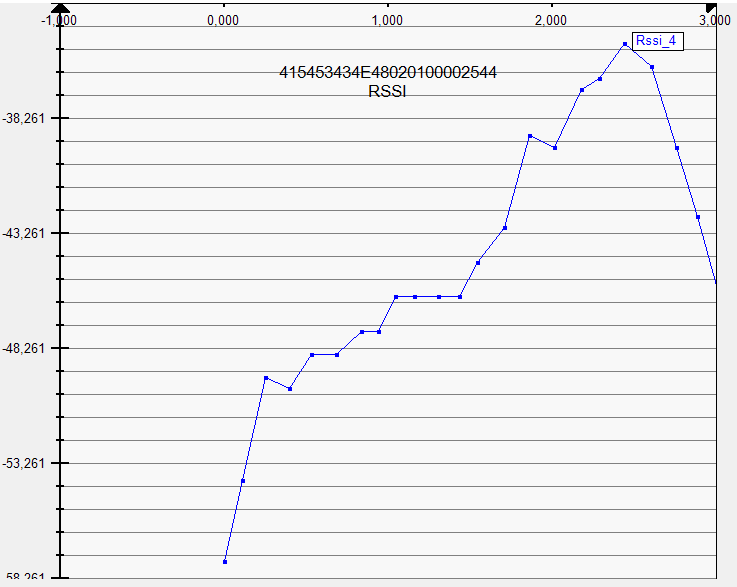
\includegraphics[width=\linewidth]{5c_in_RSSI}
\end{minipage}
\hfill
\begin{minipage}{0.42\textwidth}
	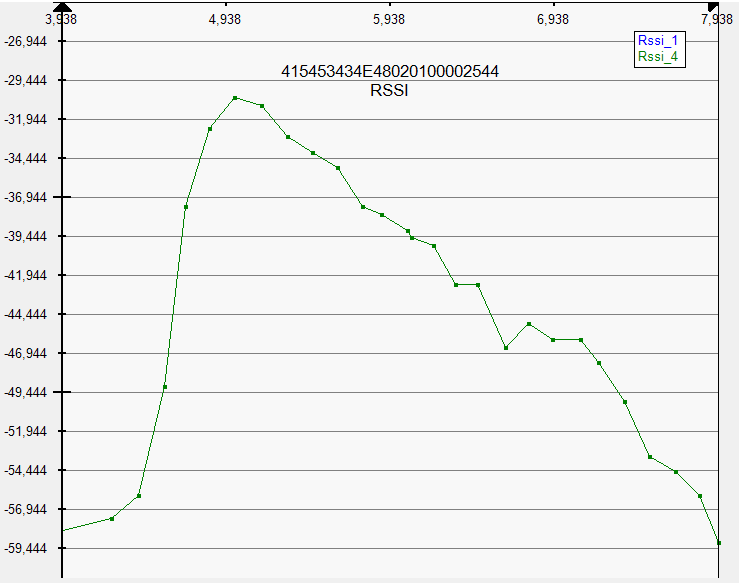
\includegraphics[width=\linewidth]{5c_uit_RSSI}
\end{minipage}

\paragraph{Testconclusie}
Het vermoeden dat de resultaten beter zijn als er verder op de lijn voor de antenne wordt gewandeld lijkt te zijn bevestigd met deze test.

\subsubsection{Deelconclusie}
In ideale omstandigheden blijkt dit concept zeer goed te werken, echter zijn er enkele neveneffecten van een realistische draai door een deur die moeten gecompenseerd worden met een langere lengte op de lijn voor de antenne te lopen. De vooropgestelde hypothese is dus niet correct en moet aangevuld worden met deze nieuwe informatie. In praktijk wilt dit zeggen dat dit niet werkt voor een normale deuropening en vorige opstelling dus gebruikt zal moeten worden. Echter kan het wel een oplossing zijn voor een (korte) gang of dergelijke waar de assets sowieso door moeten om een berging of magazijn te bereiken, want vanaf er enige afstand wordt gedaan werkt dit wel zeer goed. 

\subsection{1 tag aan deurlijst}
\subsubsection{Deelhypothese}
Deze opstelling is in staat om verspreide, getagde assets te detecteren en eenduidig een locatie toe te wijzen.

\subsubsection{Test 1: Ideale situatie}
De opstelling voor deze test is als volgt: Een rijdende kar is voorzien van een RFID-reader, of meer bepaald een vlakke antenne, welke opzij (rechts) is gericht. Verder is er een een locatie, bestaande uit 1 ommuurde ruimte, deze is voorzien van 1 locatie tag (Tagcode 4) aan het deurframe, langs de rechterkant (zodat de antenne op de kar de tag kan lezen bij het binnenkomen). Vervolgens bevinden zich verspreid over deze ruimte 4 assets (Tagcode 1, 2, 3 en 5), getagd met een asset tag. Als laatste is er aan de deurlijst aan de linker kant ook een locatie tag (Tagcode 6) aangebracht, voor een andere locatie dan deze. In en opstelling in productie zou deze aan de deur van een nieuwe locatie hangen, maar in deze opstelling is zijn functie louter om aan te geven wanneer de locatie wordt verlaten. Alle tags (zowel locatie als asset) bevinden zich op dezelfde hoogte als de antenne op de kar. De test is geslaagd als alle asset tags gemeten worden tussen het meten van eerst de locatie tag van de locatie zelf eenderzijds en, en de tag van de andere locatie anderzijds.

\paragraph{Resultaat}
De resultaten van deze test zijn ondergebracht in volgende grafiek. Met leesbaarheid in gedachten zijn de tijdsspannes tussen de registraties van de tags weggelaten uit de grafiek, in praktijk liggen deze verder uit elkaar in de tijd maar de volgorde is hier voornamelijk van belang. We kunnen zeer duidelijk zien dat deze test geslaagd is, we registreren eerst tag 4, welke duidelijk maakt dat we ons vanaf hier binnen de locatie bevinden. Elke asset tag die tussen dit moment, en het moment dat een andere locatie tag wordt gedetecteerd, ligt in deze locatie. De 2e locatie tag is de laatste die we detecteren dus er is correct bepaald dat alle assets zich in deze locatie bevinden. Wel zien we een groot verschil in aantal meetpunten, tag 5 wordt zo maar 2x gedetecteerd, in vergelijking tot de meer dan 50 meetpunten voor tag 3. Dit is echter niet geheel verrassend, aangezien het asset met tag 5 veel dieper in de kamer lag dan asset 3.

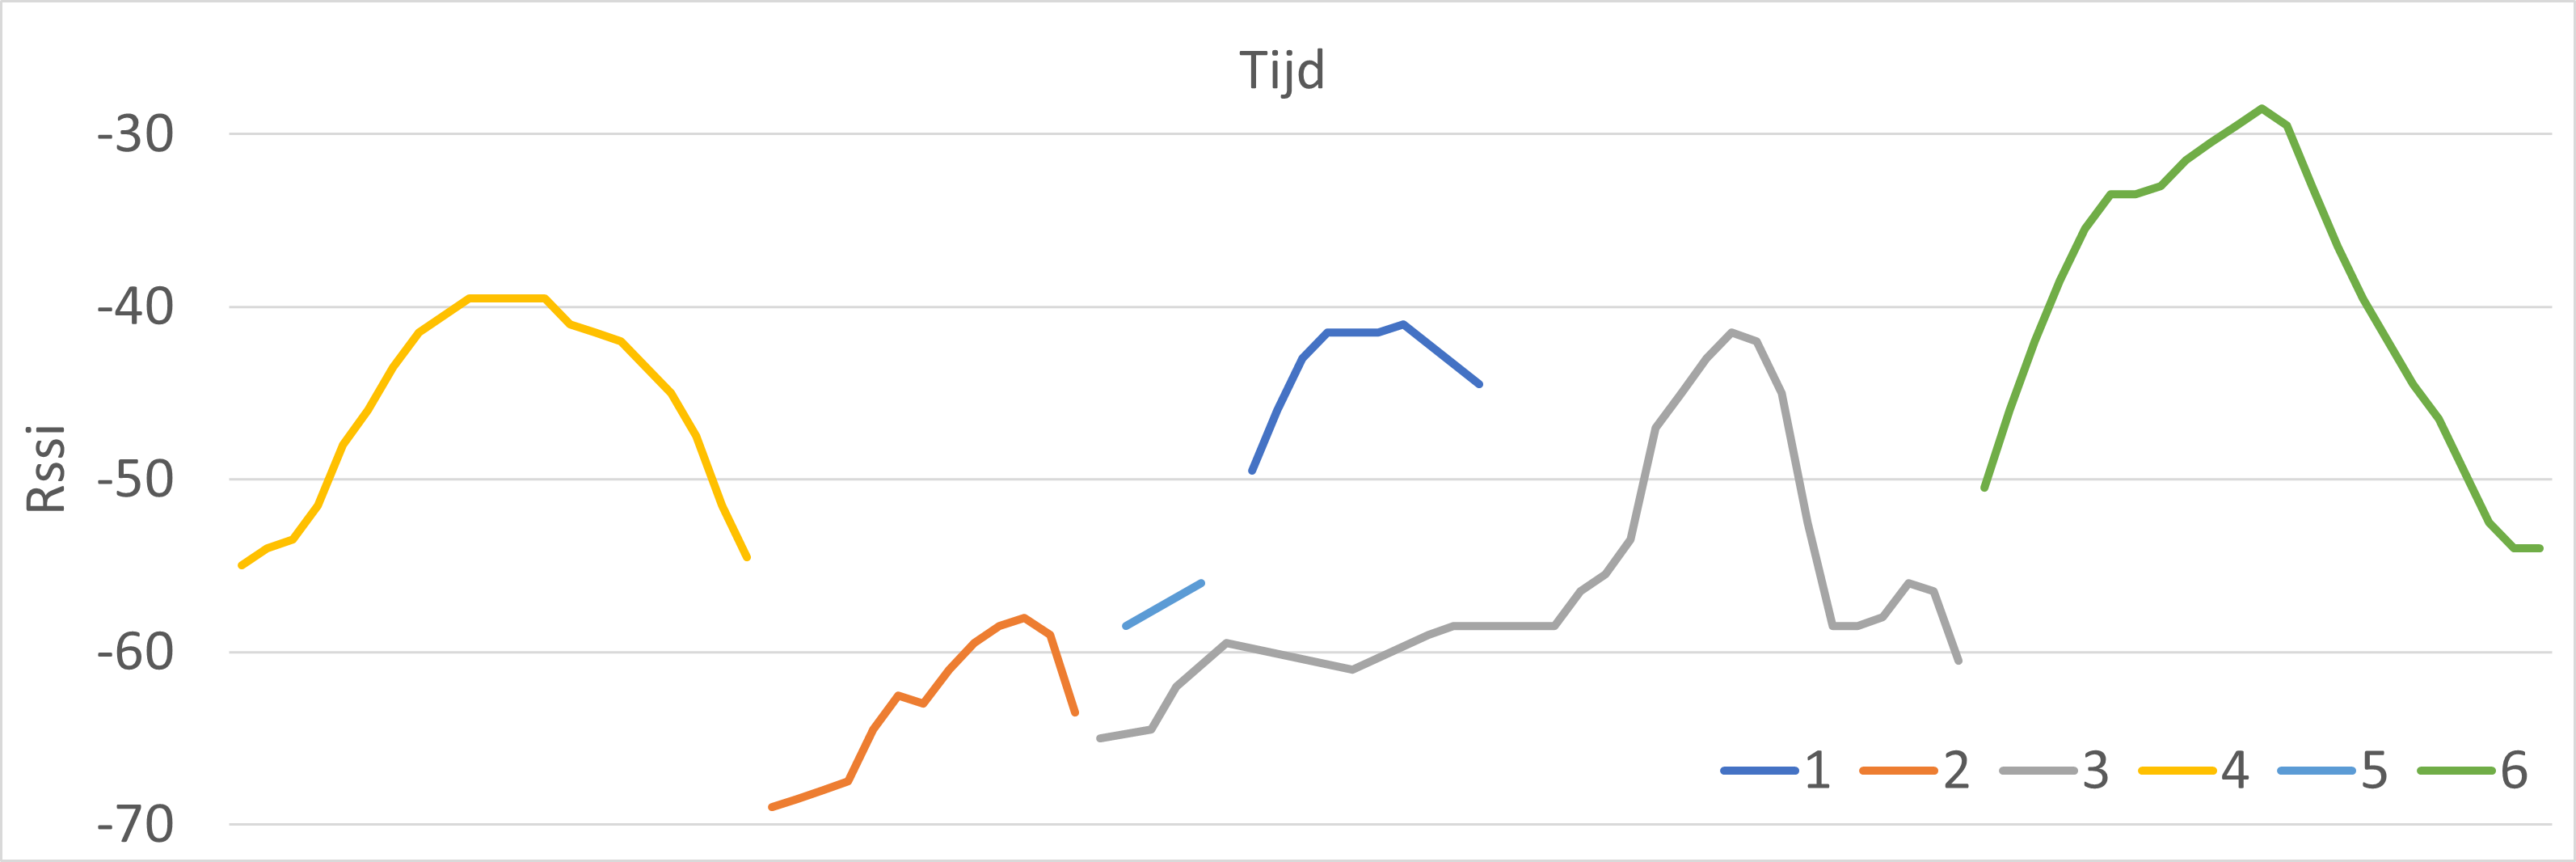
\includegraphics[width=\linewidth]{6a_RSSI}

\paragraph{Testconclusie}
Het doel van de test, namelijk het detecteren van alle assets en ze correct plaatsen in de locatie is geslaagd. Het feit dat er een groot verschil bestaat in het aantal meet- of detectiepunten wekt wel het vermoeden dat het voornaamste probleem met dit scenario zal liggen in het detecteren van alle aanwezige assets, en niet zo zeer in het bekomen van een correcte lokalisatie.

\subsubsection{Test 2: Realistische situatie}
In tegenstelling tot vorige situatie is het natuurlijk geen gegeven dat alle asset tags zich ook op ruwweg dezelfde hoogte als de antenne zullen bevinden aangezien assets zelf zich in theorie overal in de kamer kunnen bevinden, inclusief op tafels of kasten. Deze test zal dus dezelfde opstelling nemen als de vorige test, maar de assets zullen zich ook op verschillende hoogtes bevinden.

\paragraph{Resultaat}
Dit resultaat toont de vrees van vorige test aan, de detectie is helaas veel slechter als de tags niet op het niveau van de antenne liggen. De volgorde is nog steeds correct, dus qua lokalisatie is er geen probleem. Echter is bij elke asset tag het aantal meet- of detectiepunten afgenomen en is de RSSI gezakt. Tag 5 is zelfs volledig verdwenen uit de data en is dus niet gedetecteerd.

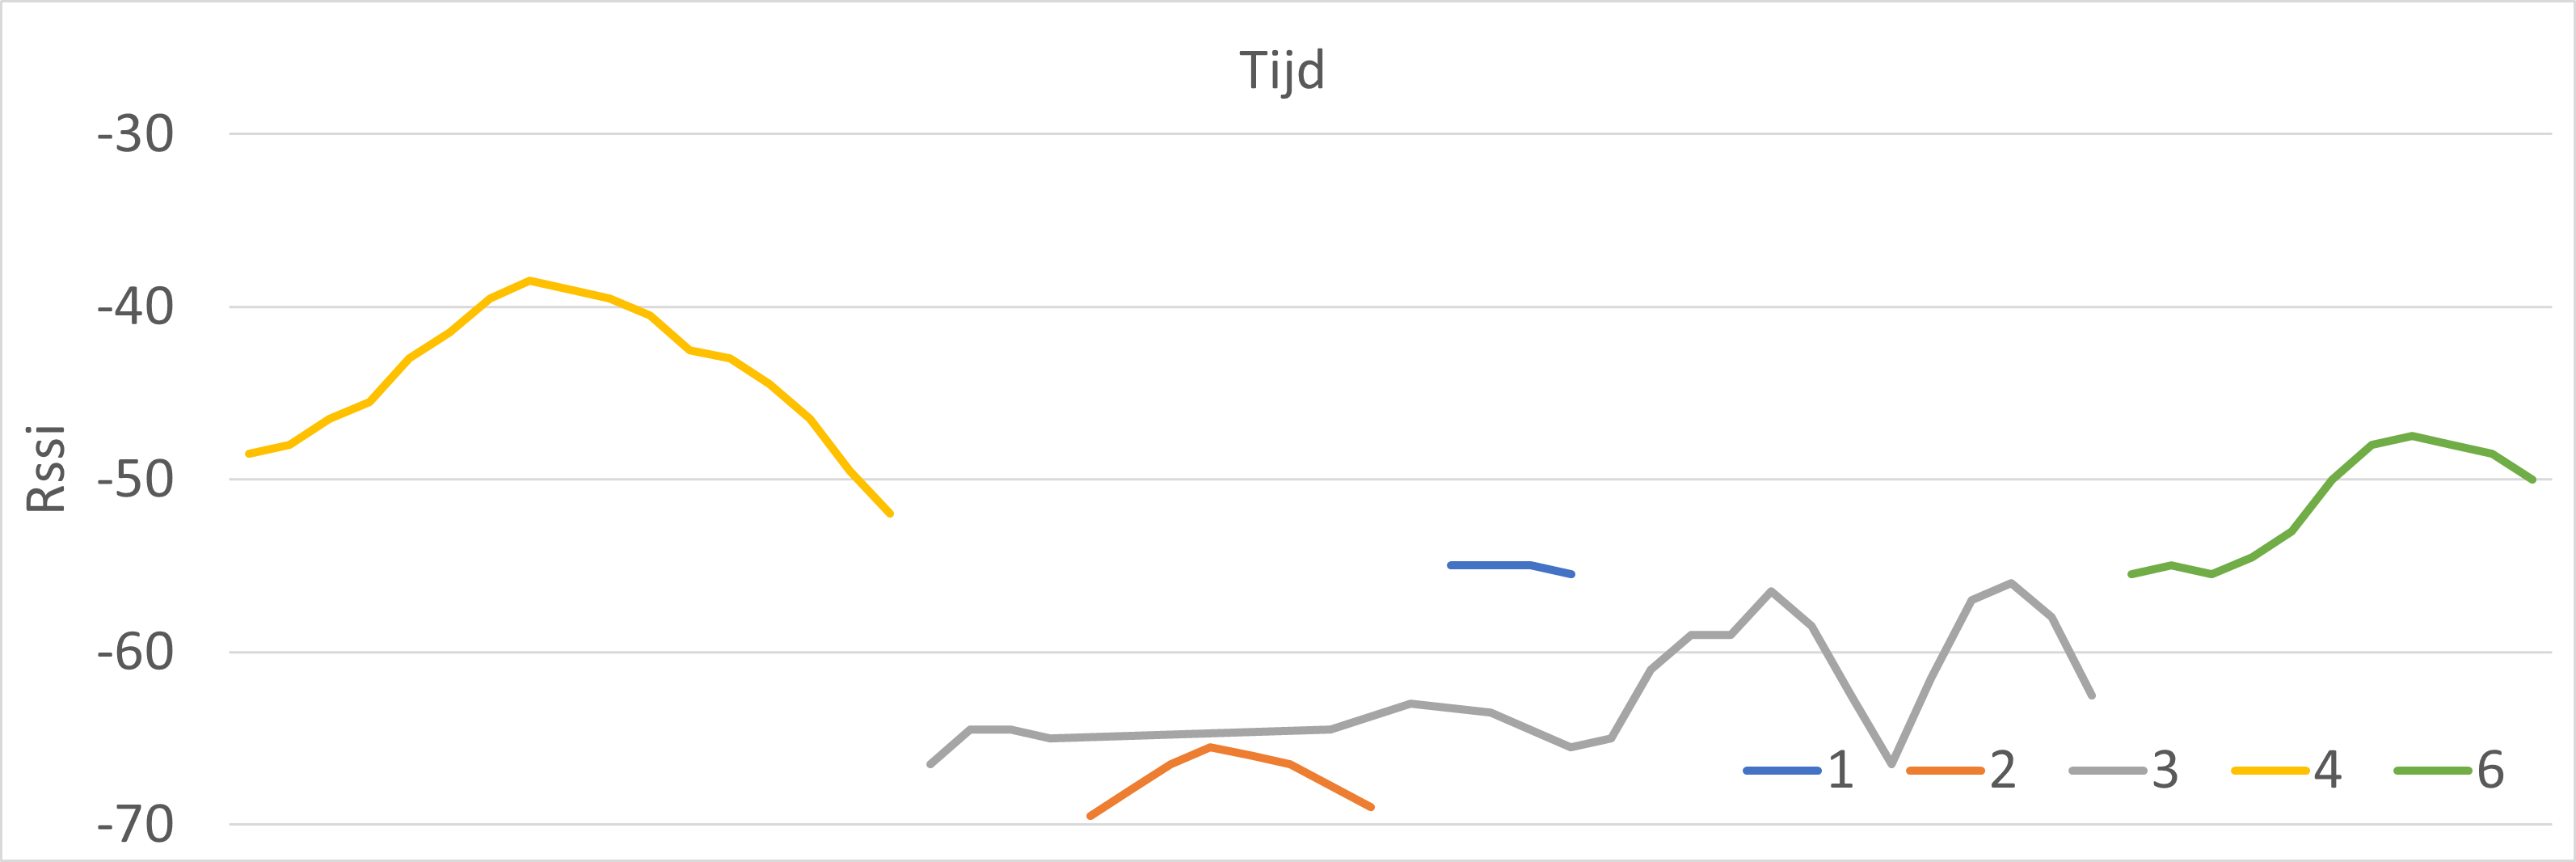
\includegraphics[width=\linewidth]{6b_RSSI}

\paragraph{Testconclusie}
Als de asset tags niet meer op hetzelfde niveau liggen als de antenne, is hun detectie dus veel minder. Dit hoeft echter niet zo'n zeer probleem te zijn aangezien 1 meetpunt in theorie voldoende is om te weten dat het asset aanwezig is, een tag die niet aanwezig is op de locatie zal uiteraard ook niet 1x antwoorden. Wel is het wegvallen van tags een probleem, want dan kan bijhorend asset niet gelokaliseerd worden, en deze kans wordt groter als de detectie verslecht.

\subsubsection{Deelconclusie}
Qua lokalisatie blijkt dit concept perfect te werken, echter is dit logisch gezien ook niet verrassend. Het voornaamste probleem is het kunnen detecteren van alle aanwezige tags, wat met een RFID opstelling niet vanzelfsprekend is. Uiteraard is het mogelijk om met een andere hardwareopstelling, bv. antennes op verschillende hoogtes, of een staafantenne met een ander bereikveld dan een vlakke antenne, mogelijk om betere detectie te bekomen. Echter evolueert dit op deze manier in een RFID detectieprobleem en komt daarmee buiten de scope, nl. lokalisatie, van dit onderzoek te liggen. Verder is er binnen Aucxis voldoende ervaring op dit veld dat verder onderzoek nutteloos zou zijn.

\section{BLE}

\subsection{Vooronderzoek}
Voordat overgegaan kan worden naar het onderzoeken van de opstellingen die gebruik maken van BLE, is het nodig enkele testen te doen om het gedrag van BLE vast te stellen, en om enkele veronderstellingen te testen.

\subsubsection{Test 1: Variatietest}
Aangezien de lokalisatieopstellingen verder in dit hoofdstuk gebruik zullen maken van RSSI waardes om de locatie van de beacons, en dus ook de bijhorende assets, te bepalen, is het belangrijk dat deze waardes constant zijn in de tijd als alle andere variabelen constant zijn. 
Voor deze test worden de gateway en de beacon op een afstand van 150cm uit elkaar gelegd, in hetzelfde vlak. Vervolgens wordt over lange tijd de RSSI waardes gemeten. Dit experiment wordt uitgevoerd bij 3 en bij 30 beaconberichten per gatewaybericht, dit om te bekijken of dit een effect heeft. Want logischerwijs zal ook deze verhouding een invloed hebben, nl. hoe meer berichten de gateway heeft ontvangen, hoe meer de eventuele extreme waarden zullen uitgemiddeld worden en hoe stabieler de waarden uitgestuurd door de gateway zullen worden.
Beide experimenten zijn uitgevoerd met 5 verschillende beacons van het type MokoSmart H5, en 2 beacons van het type MokoSmart M2. Ze zijn allen aangeduid a.d.h.v. de laatste 2 karakters van hun MAC adres.

\paragraph{a) 3 beaconberichten per gatewaybericht}
Uit dit testresultaat is duidelijk af te lijden dat een uitmiddeling van 3 berichten een zeer grote variatie veroorzaakt in de RSSI waarden, met bij bv. beacon FB een verschil tussen de uitersten van 14 dBm. Aangezien de FSPL formule duidelijk maakt dat in theorie een verschil van 6 dBm een verdubbeling van de afstand betekend, komt deze onzekerheid neer op een afstandsverschil van ongeveer factor 4, het spreekt voor zich dat dit nefast is voor elke poging tot lokalisatie.

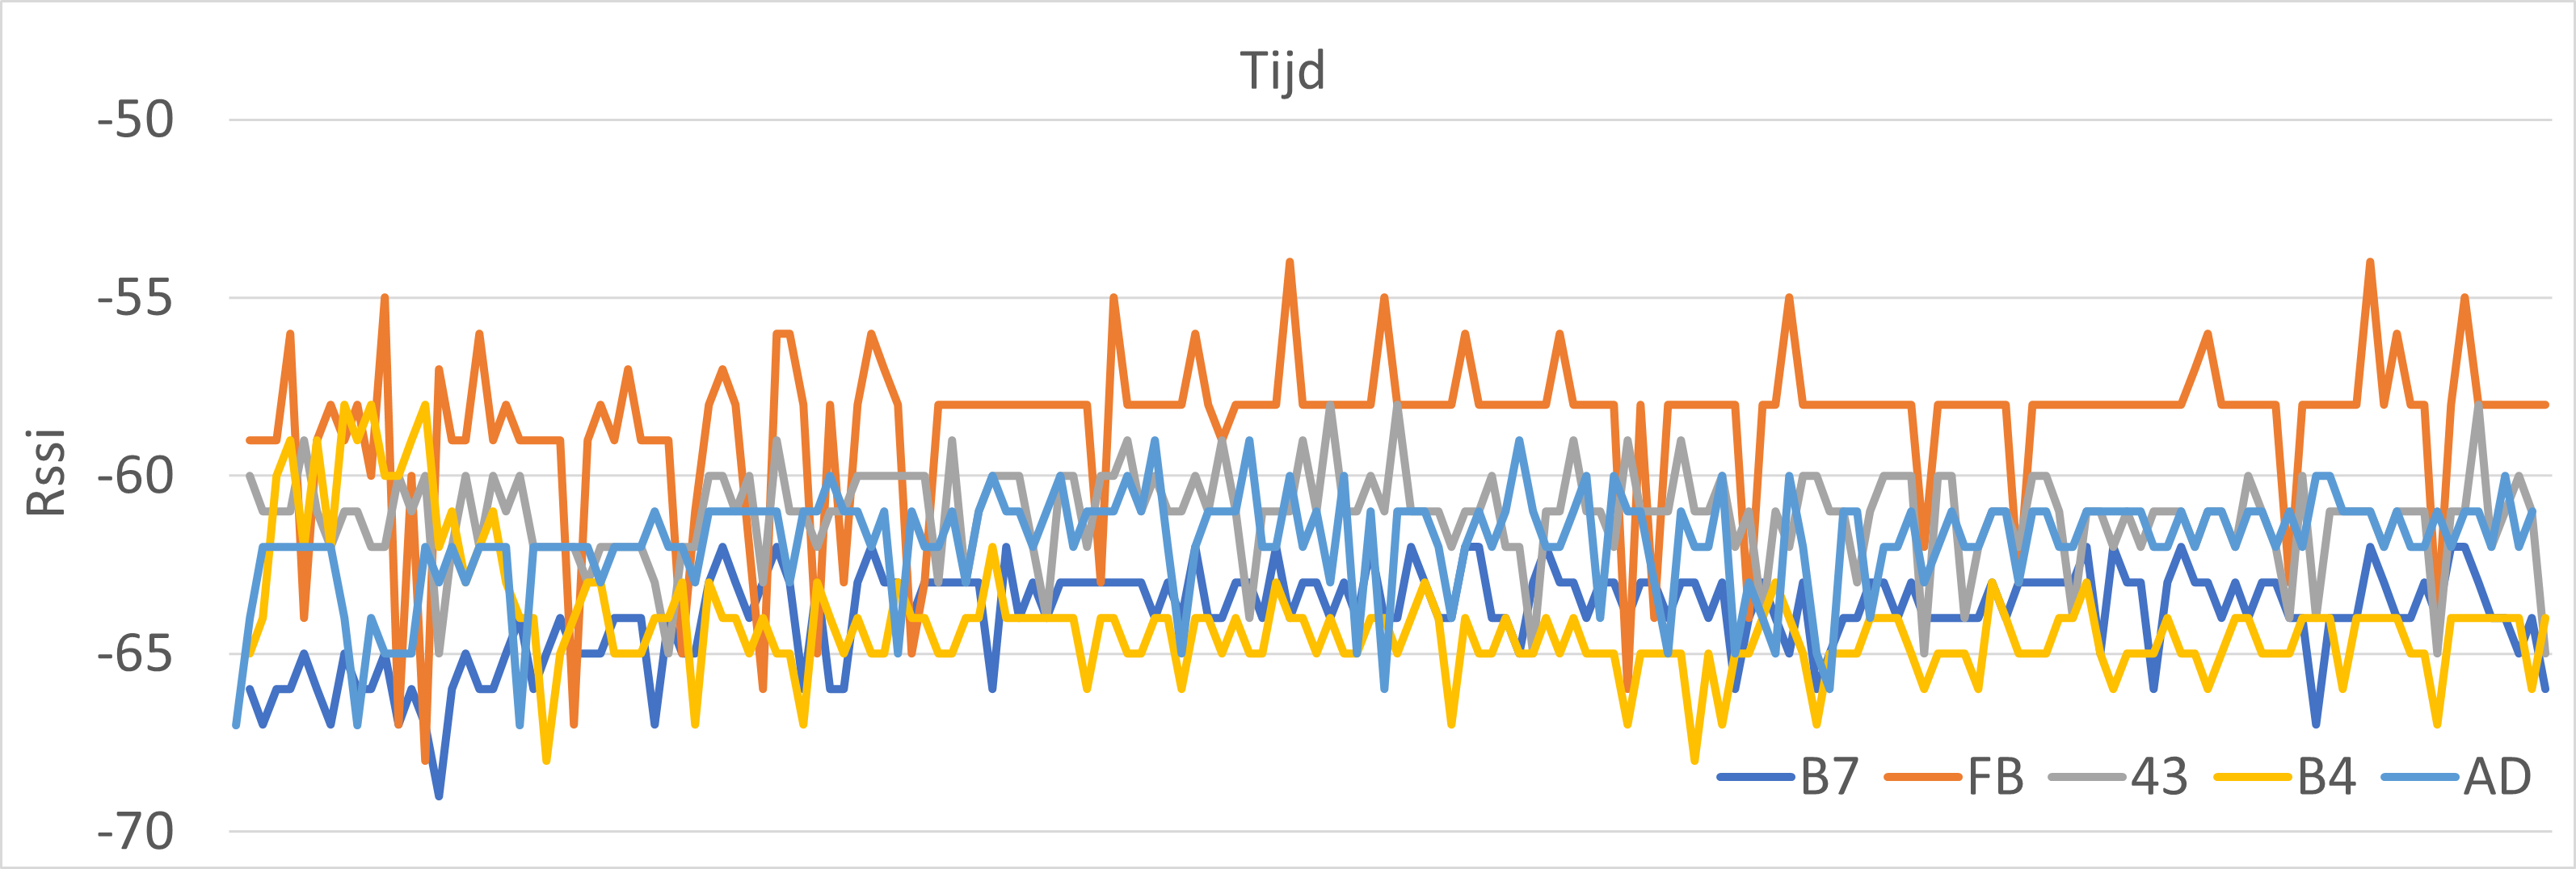
\includegraphics[width=\linewidth]{sble_0_1a}

\paragraph{b) 30 beaconberichten per gatewaybericht}
Uit deze test is zichtbaar dat een uitmiddeling over 30 berichten veel minder variatie geeft, met over het algemeen een variatie van plus en min 1 van de gemiddelde waarde. Dit lijkt meer acceptabel. Ook is er in dit experiment 1 H5 beacon (code AD) vervangen door 2 beacons van het type H2. Dit om een vermoeden te onderzoeken dat, alhoewel alle beacons dezelfde instellingen hebben, hun zendsterkte toch varieert. Dit is hier ook bevestigd, deze 2 (6F en 23) hebben een hogere gemiddelde RSSI waarde dan de 4 overgebleven H5 beacons, welke onderling ook vrij veel van elkaar verschillen.

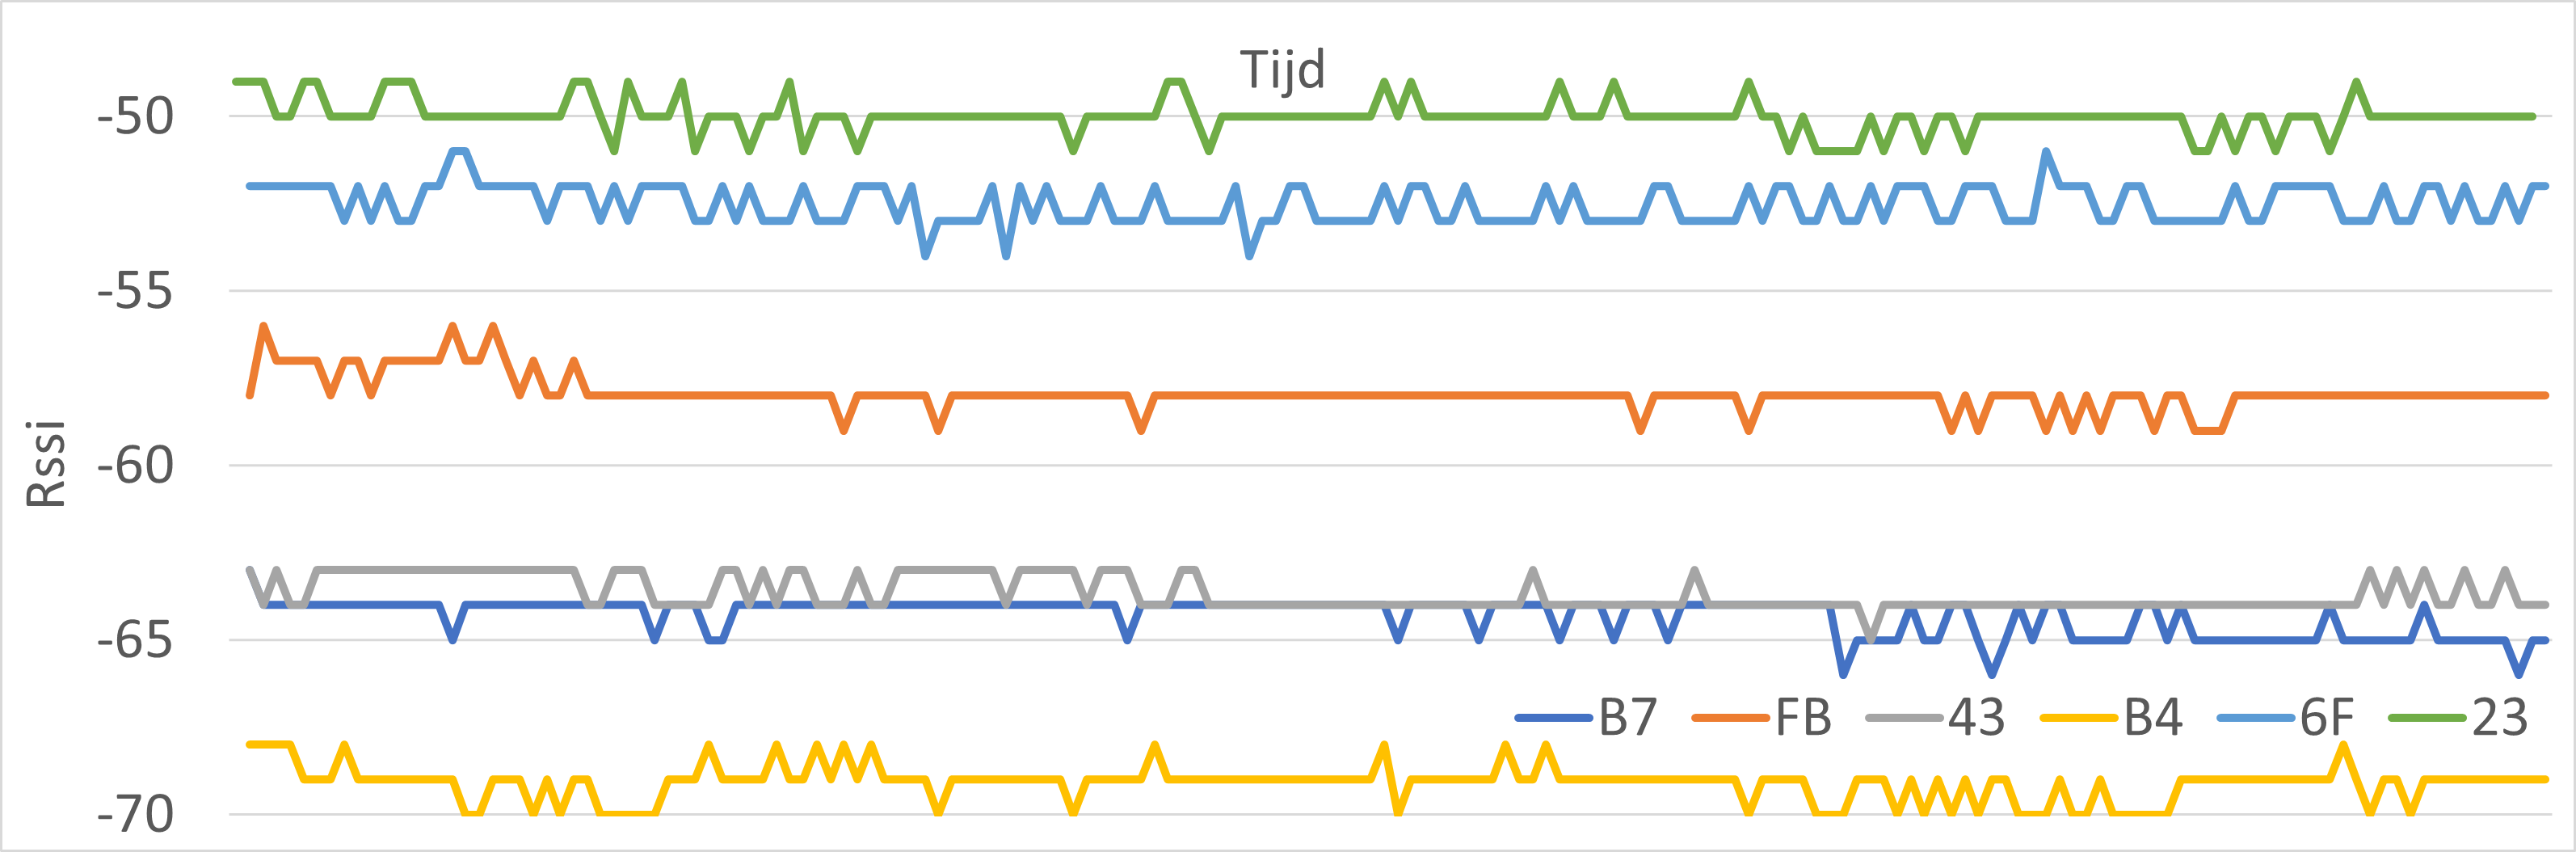
\includegraphics[width=\linewidth]{sble_0_1b}

\paragraph{Testconclusie}
Uit deze eerste test zijn 2 dingen duidelijk geworden, allereerst dat er een goed aantal beaconberichten nodig is voor uitmiddeling per gatewaybericht, anders zijn er grote variaties in de RSSI waarden. Aan het versnellen van de beacons is echter ook een groot nadeel verbonden, namelijk het verminderen van de batterijduur. Deze factor is rechtstreeks verbonden aan kostprijs, voor de nieuwe batterij, en de werkuren om deze te vervangen. Ook zal het afhangen van de use-case hoe belangrijk deze is. Alternatief kan ook de gateway trager uitsturen, wat een negatief effect zal hebben op de lokalisatiesnelheid. Dit zal een afweging zijn gebaseerd op de situatie maar is zeker niet onbelangrijk. Tijdens het verdere verloop van dit onderzoek zal een (arbitraire) waarde van 30 beaconberichten per gatewaybericht worden aangehouden, aangezien dit een mooie middenweg lijkt, maar dit kan duidelijk verhoogd/verlaagd worden met de voor- en nadelen vandien.

Als 2e is er ook duidelijk geworden dat er een verschil zit tussen de zendsterkte van BLE beacons met dezelfde instellingen. Dit zowel voor beacons van hetzelfde type, als van andere types. Hieruit volgt dus dat, als er een omzetting van RSSI waarde naar een afstand moet worden gemaakt, deze waarde op een of andere manier zal moeten worden genormaliseerd. Een mogelijkheid hiervoor is het veld 'RSSI at 0m', aanwezig in een UID bericht. Een andere optie is de beacons kalibreren dat ze even sterk zenden. Ongeacht hoe hier rond wordt gewerkt, blijft het een aandachtspunt.

\subsubsection{Test 2: Afstandstest}
De volgende veronderstelling die zal worden getest, is het verloop van de RSSI waardes, in functie van afstand tussen de beacons en de gateway. In theorie zou deze moeten verlopen volgens de FSPL formule (ongeveer exponentieel, met en neerwaarts traject van ~6dBm per verdubbeling van de afstand). Deze test heeft als doel na te gaan of dit in praktijk ook zo is.
In dit experiment zal een gateway worden opgesteld, met een beacon die steeds verder van deze gateway zal verwijderd worden in intervallen van 50cm. Dit experiment zal 3x worden herhaald, 1x in een ideale omgeving, nl. een anechoïsche kamer\footnote{Een anechoïsche kamer is een kamer waarvan de muren bedekt zijn met speciaal gevormd mousse, meestal puntvormig. Dit is bedoeld om radio- en geluidsgolven zo goed mogelijk te absorberen en zo een kamer te creëren met zo weinig mogelijk reflecties.}, 1x in een open reële omgeving, nl. een bemeubelde huiskamer, en ditzelfde nogmaals, maar met 1 muur tussen, om zo het verwachte negatieve effect van obstakels te controleren. De meting in ideaal geval zal minder meetpunten bevatten dan de reële, omwille van de gelimiteerde grootte van de anechoïsche kamer.

\subsubsection{Resultaat}
Er is duidelijk zichtbaar dat theorie en realiteit veel van elkaar verschillen. De (beperkte) meetpunten van de ideale meting komen zeer goed in de buurt van de theorie, maar vanaf er wordt overgestapt naar een open reële ruimte zijn de resultaten zeer anders. Met als voornaamste bevindingen dat de waarden veel lager liggen dan in theorie, en dat het niet elke waarde dalend is. Wel is aan de bijgetekende logaritmische trendlijn te zijn dat de reële waarden wel een dalend verloop kennen. Verder zien we dat ook de meting met muur een grillig, maar neerwaarts verloop vertoon, op een lager niveau dan zonder muur.

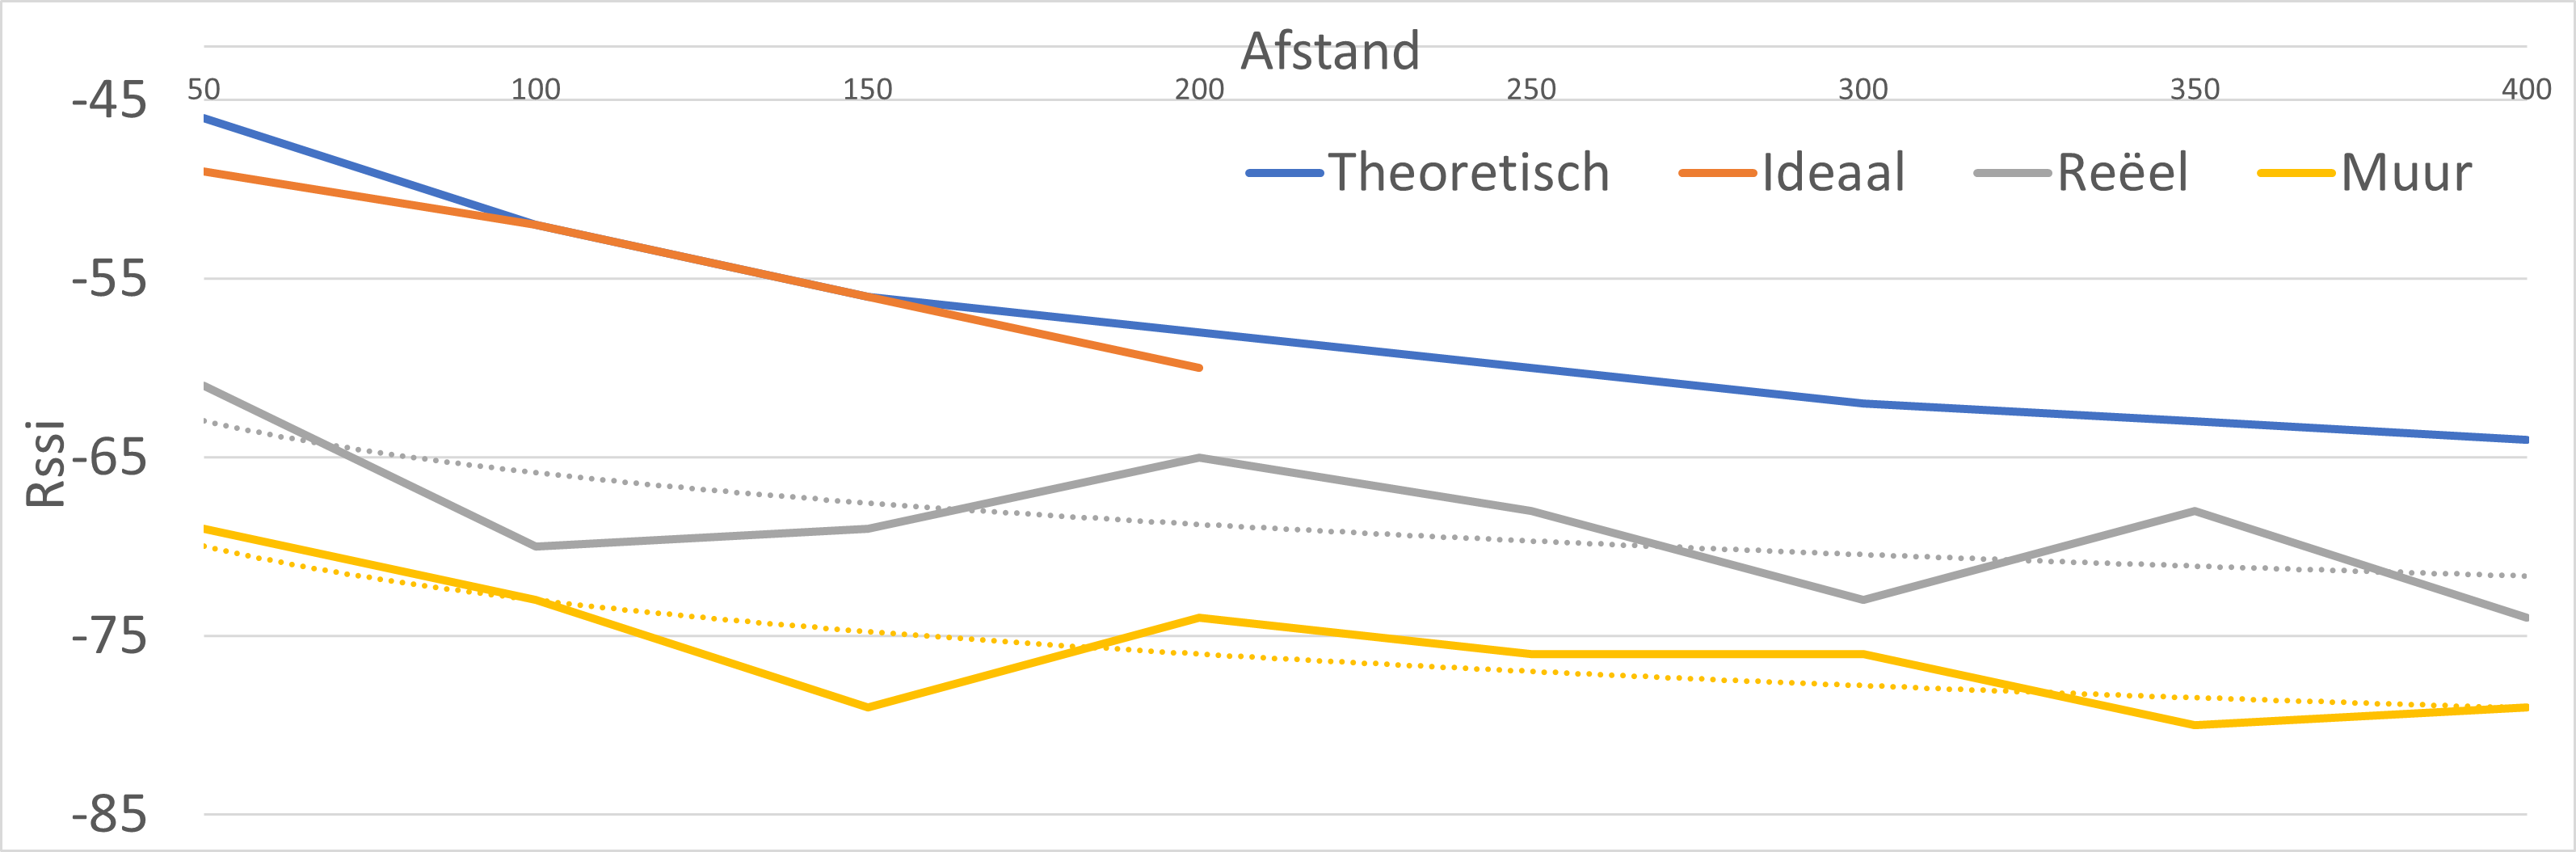
\includegraphics[width=\linewidth]{sble_0_2}

\emph{De reële testen zijn uitgevoerd met 5 verschillende MokoSmart H5 beacons, echter aangezien allen een gelijkaardig verloop vertoonden, worden de andere 4 niet extra bijgevoegd.}

\paragraph{Testconclusie}
Aangezien het voornaamste verschil tussen de ideale en realistische situatie het bestaan van reflecties is, is met deze test dus duidelijk geworden dat deze een zeer grote impact kunnen hebben op de resultaten en de RSSI waarden. Voornamelijk in de vorm van een schommeling, welke vervelend is als er een conversie moet worden gemaakt tussen RSSI en afstand, en verder ook in een algehele RSSI vermindering tegenover de theorie. 
De testen voor de effectieve scenario's zullen allen plaatsvinden in reële omgevingen, aangezien implementaties van systemen gebaseerd op deze scenario's ook in reële ruimtes zullen werken, en puur theoretische of ideale situaties dus geen nut hebben om te vergelijken.

\subsubsection{Test 3: Rotatietest}
Deze derde en laatste test in dit vooronderzoek zal de veronderstelling testen dat de meting van de gateway richtingsonafhankelijk is, nl. of er een verschil is in RSSI als de enige variabele de locatie van de beacon rond de gateway is.
Voor deze test is een gateway opgesteld op een draaiplatform in een anechoïsche kamer, met een MokoSmart H5 beacon op 150cm afstand. Tijdens te test zal de gateway rond zijn as draaien. Dit gebeurt 2x, eens met de beacon op dezelfde hoogte als de gateway, en eens met de beacon 50cm hoger.

\paragraph{a) Beacon en gateway op zelfde hoogte}

\begin{minipage}{0.55\textwidth}
Uit dit resultaat is zeker duidelijk dat er een zekere richtingsafhankelijk is, met een grote blindspot rond 260° van -68 dBm, een verschil met het gemiddelde van 10dBm, met 2 kleinere op 80° en 180° met een verschil van 5 dBm. Alhoewel niet drastisch, het overgrote deel van is vrij constant, is dit toch noemenswaardig. De meest voor de hand liggende verklaring hiervoor is het feit dat de ingebouwde (staaf) antenne loopt op de lijn van 90° en 270°, dus de 2 voornaamste dippen wijzen ongeveer naar de uiteinden van deze antenne, en een blindspot hier is karakteristiek voor een staafantenne.
\end{minipage}
\hfill
\begin{minipage}{0.42\textwidth}
	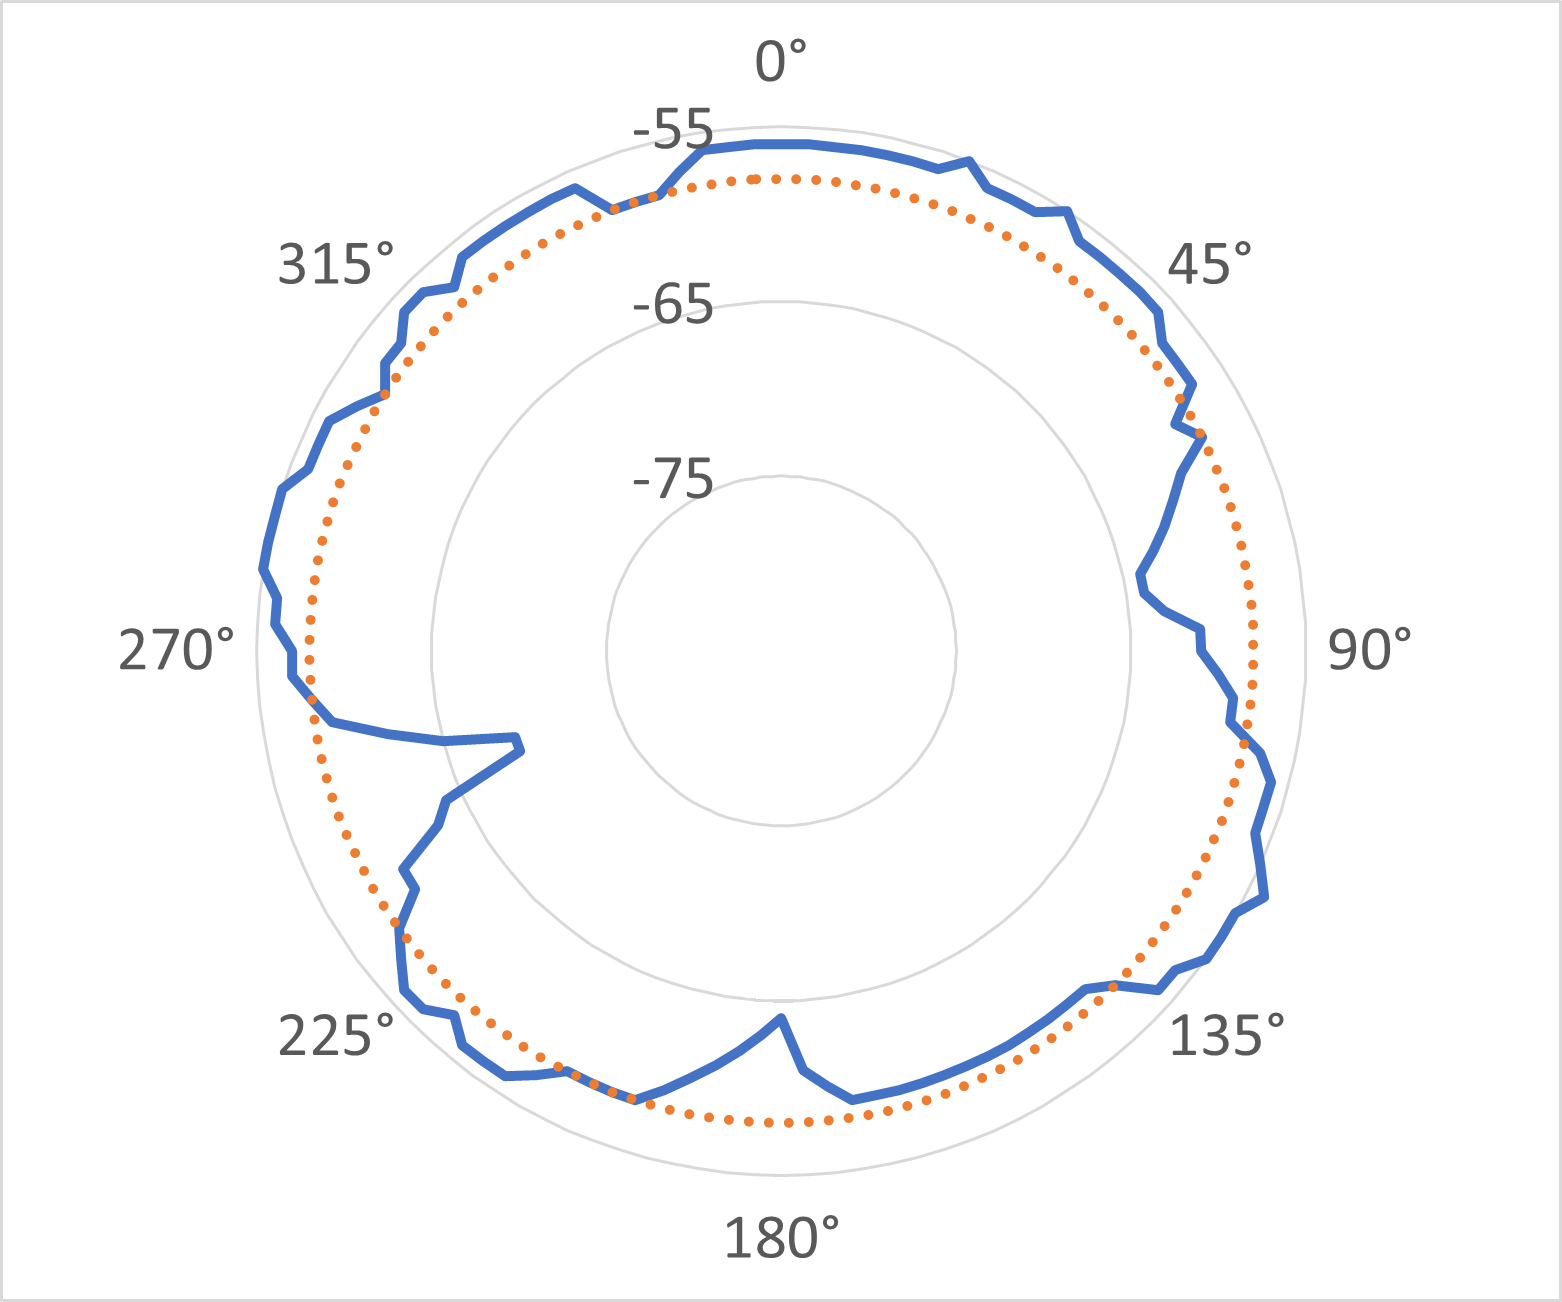
\includegraphics[width=\linewidth]{sble_0_3a}
\end{minipage}


\paragraph{b) Beacon 50cm boven gateway}

\begin{minipage}{0.55\textwidth}
Hier is zichtbaar dat de harde blindspots uit de vorige test verdwenen zijn, wat het vermoeden dat dit met de antennerichting te maken heeft lijkt te bevestigen. Wel is er nog een duidelijk dal in het kwartaal tussen 225° en 315°.
\end{minipage}
\hfill
\begin{minipage}{0.42\textwidth}
	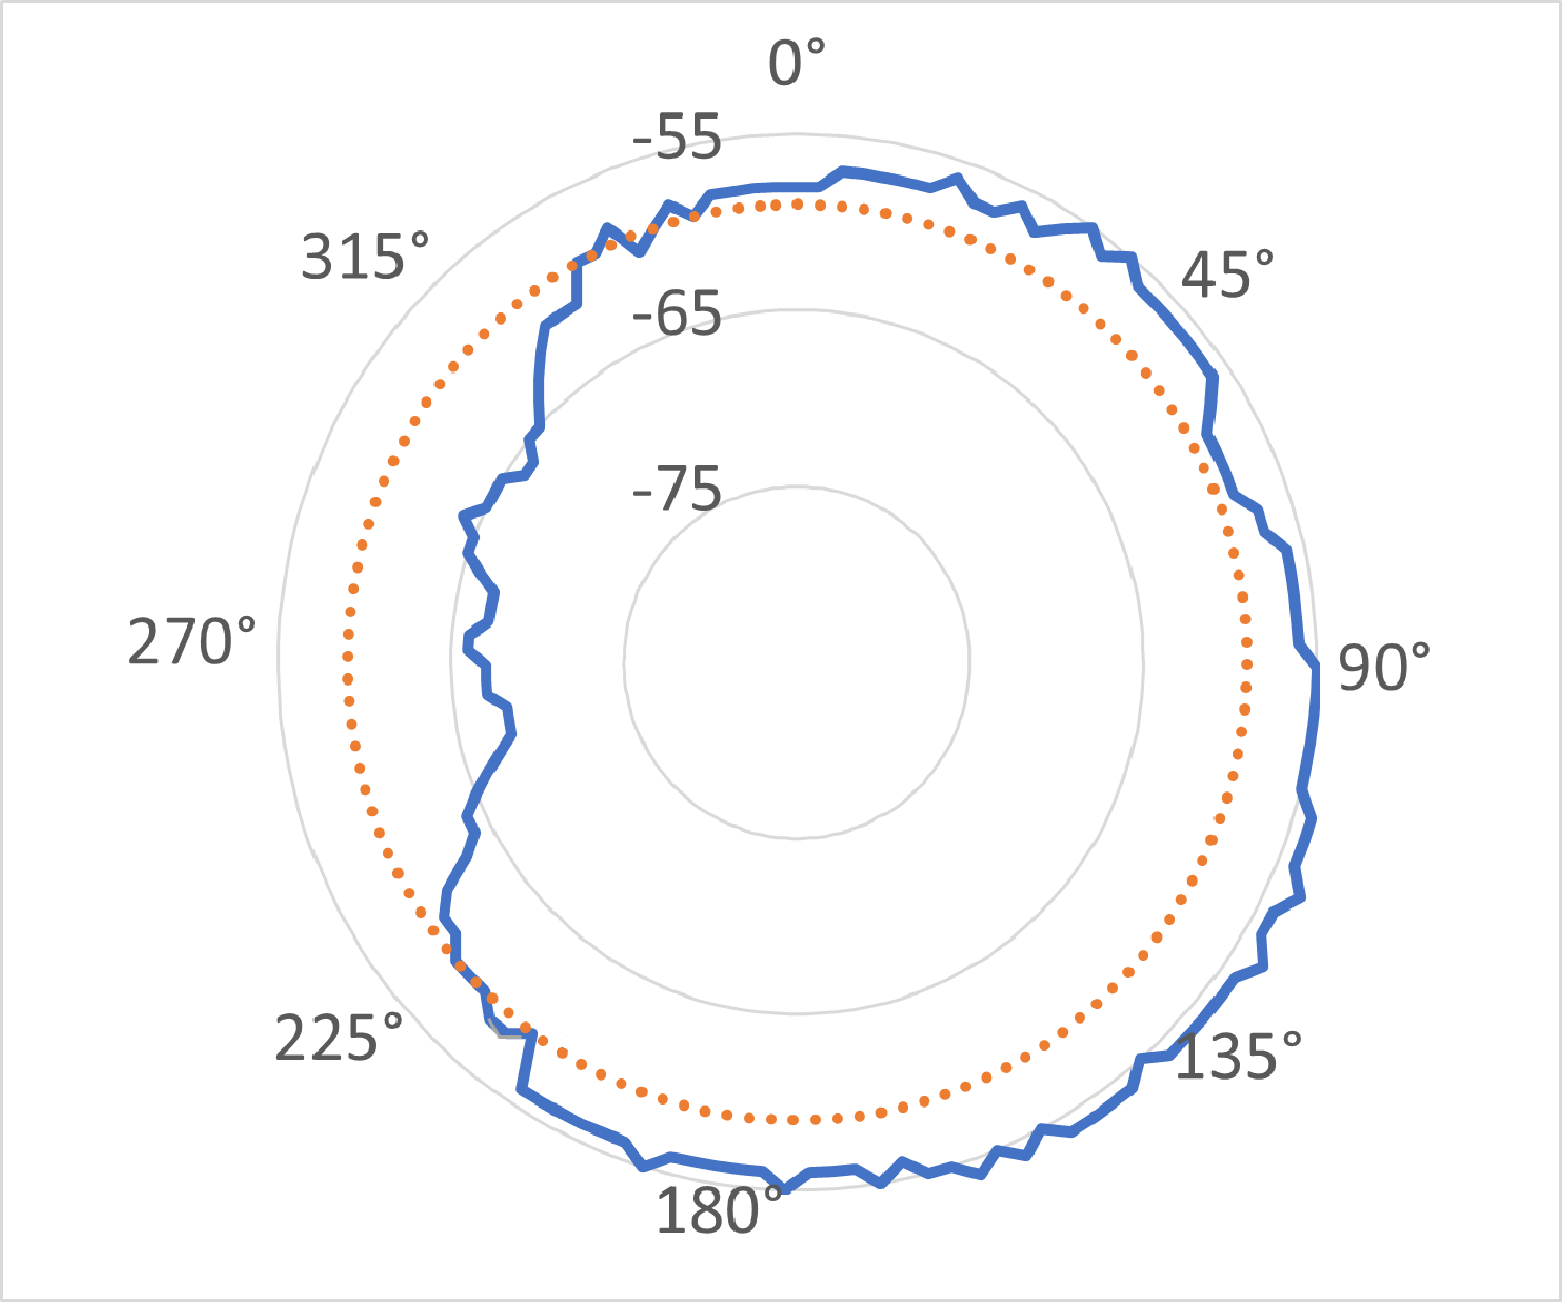
\includegraphics[width=\linewidth]{sble_0_3b}
\end{minipage}

\paragraph{Testconclusie}
Uit deze test is duidelijk geworden dat een gateway niet 100\% richtingsonafhankelijk is. Over de grote lijn zal dit vermoedelijk geen problemen geven, echter kunnen de plotse daten in meetgevoeligheid onverwachte waarden opleveren als een beacon toevallig net in die richting ligt.
Tijdens de volgende testen zullen alle gateways in dezelfde richting worden geplaatst om het effect van deze verlopen te standaardiseren. 

\subsubsection{Deelconclusie}
Uit dit vooronderzoek is duidelijk geworden dat niet elke theoretische veronderstelling ook geldig is in een reële praktijk. Het is belangrijk dit eerst vastgesteld te hebben, aangezien het waarschijnlijk mogelijk zal zijn om sommige anders onverklaarbare fenomenen in komende scenariotests te verklaren. Ook zijn er in de testconclusies maatregelen/standaarden vastgelegd om deze effecten zo veel mogelijk te standaardiseren.

\subsection{1 gateway per locatie}
\subsubsection{Deelhypothese}
Deze opstelling zal een asset kunnen lokaliseren, genomen dat de gekozen locaties een gelijkaardige grootte hebben.

\subsubsection{Test 1: 6 locaties in reële, open ruimte, gelijk verdeeld}
\begin{minipage}{0.55\textwidth}
De eerste test voor deze opstelling bestaat uit de eenvoudigste en best case opstelling. In een open ruimte zijn, in een raster, 6 gateways\footnotemark geplaatst, op een afstand van 2m uit elkaar. Dan is de ruimte in 6 locaties verdeeld, volgens de afstand van de beacons. Een punt behoort dus tot de locatie van de dichtstbijliggende gateway. In praktijk komt deze locatieafscheiding\footnotemark neer op een raster middendoor de gateways. Verder worden er verschillende MokoSmart H5 en M2 beacons verdeeld over de ruimte, en zal worden bekeken waar zij volgens de gemeten waarden zich bevinden, en zal dit worden vergeleken met hun echte positie.
\end{minipage}
\footnotetext{Gateways worden aangeduid door een grijs blokje met een bijhorende letter. De illustratie is ook voorzien van 2 rode stippen op de gateway, deze illustreren de voorkant (0°) van de gateway.}
\footnotetext{De grenzen van locaties worden in de illustraties aangegeven door een stippellijn.}
\hfill
\begin{minipage}{0.42\textwidth}
	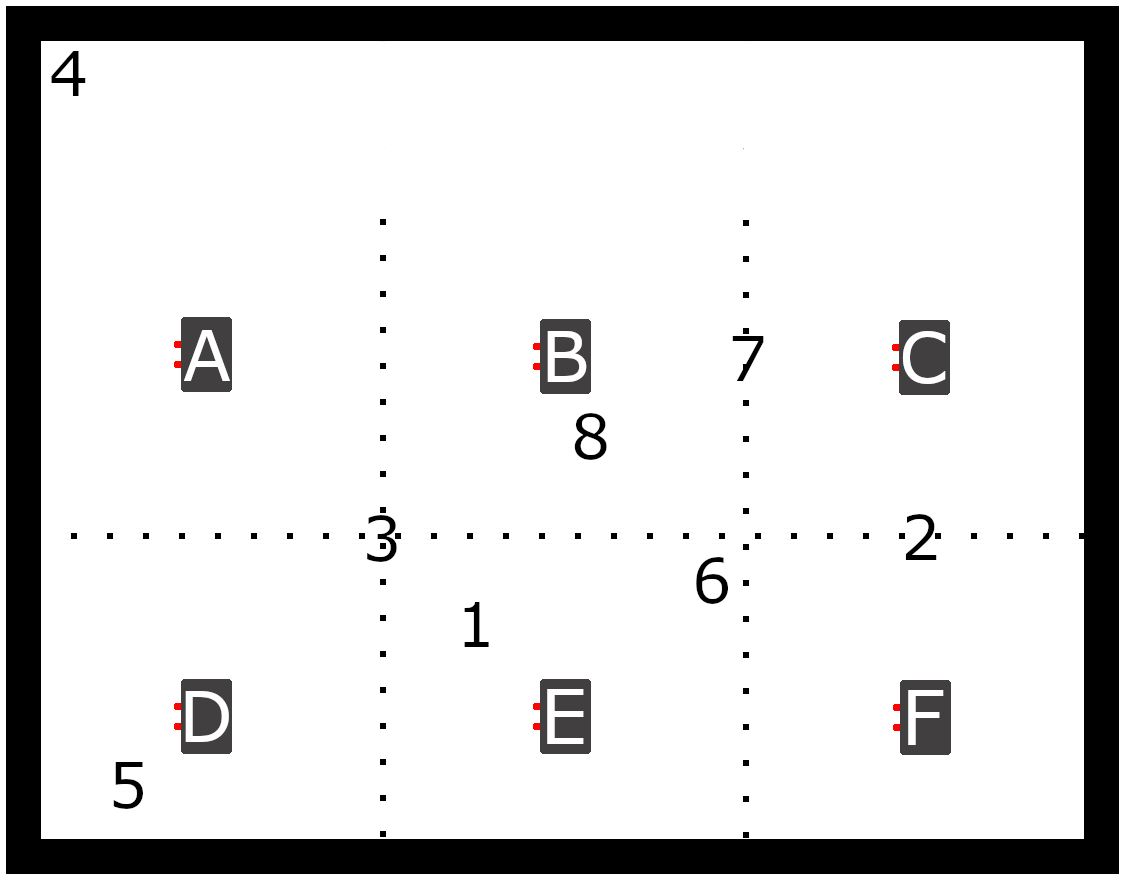
\includegraphics[width=\linewidth]{sble_1_1_floor}
\end{minipage}

\paragraph{Resultaat}
\begin{minipage}{0.55\textwidth}
De resultaten van deze test zijn zichtbaar in bijhorende tabel. De laagste waarden per beacon staan aangeduid in het groen, en het is meteen duidelijk dat deze toewijzing over het algemeen goed is verlopen. Ook grensgeval beacons zijn toegewezen aan 1 van hun aangrenzende locaties. Enkel bij beacon 6 en 8 is een verschil te vinden.
\end{minipage}
\hfill
\begin{minipage}{0.42\textwidth}
	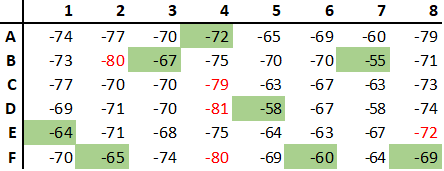
\includegraphics[width=\linewidth]{sble_1_1_results}
\end{minipage}

We hebben een onderscheid in soorten beacons die even apart horen besproken te worden, in volgorde van moeilijkheid. Allereerst hebben we beacons die duidelijk in een locatie liggen, niet tussen 2 beacons. Tijdens deze test zijn dit beacon 4 en 5. Deze zijn beiden met een comfortabel RSSI verschil gecategoriseerd in de juiste locatie. Verder hebben we de beacons duidelijk in een locatie, maar tussen verschillende gateways. Dit zijn beacons 1 en 8. Hoewel beacon 1 met voorsprong correct is, is er iets vreemd gebeurd bij beacon 8, welke gecategoriseerd wordt bij gateway F, van een zelfs niet aangrenzende locatie.  Dit is zeer vreemd aangezien deze zeer dicht bij gateway B lag, maar als we dit vergelijken met het meetpatroon van de gateway zien we dat deze toevallig net in een blindspot lijkt te liggen, wat een mogelijke verklaring zou kunnen zijn. Verder zijn er de grensgeval beacons, waaronder beacon 2 en 7, welke op de grens tussen 2 locaties liggen. Zij zijn echter toegewezen aan 1 van deze 2, welke in orde is, aangezien het in dit scenario niet de bedoeling is om een exacte positie te bepalen, maar toewijzing aan een locatie te doen. En als laatste beacon 3 en 6 op een 4-punt. Beacon 3 is ook aangrenzend toegewezen dus ook in orde. Beacon 6, alhoewel fysiek net over de grens van locatie E liggend, is toegewezen aan aangrenzende locatie F. In theorie is dit dus een fout, maar geen grote. Ook is een zekere foutmarge bij de locatiegrenzen geen verassing, gezien de onzekerheden in de RSSI waarden vastgesteld in het vooronderzoek.

\paragraph{Testconclusie}
De eerste test heeft bewezen dat dit lokalisatiescenario mogelijkheden heeft, op zijn minst in een eenvoudige egale opstelling. Een toewijzingsscore van 6.5/8 is ook zeker acceptabel.

\subsubsection{Test 2: 6 even grootte in reële, open ruimte, ongelijk verdeeld}
\begin{minipage}{0.55\textwidth}
Deze test verandert de locaties van gelijke grootte uit vorige test in locaties van variabele grootte en vorm. Verder is de ruimte, hoewel nog steeds open, niet meet convex. De locaties blijven dit wel. Hier is het dus niet zo dat elk punt zich ook bij zijn dichtstbijzijnde gateway bevind qua locatie.
\end{minipage}
\hfill
\begin{minipage}{0.42\textwidth}
	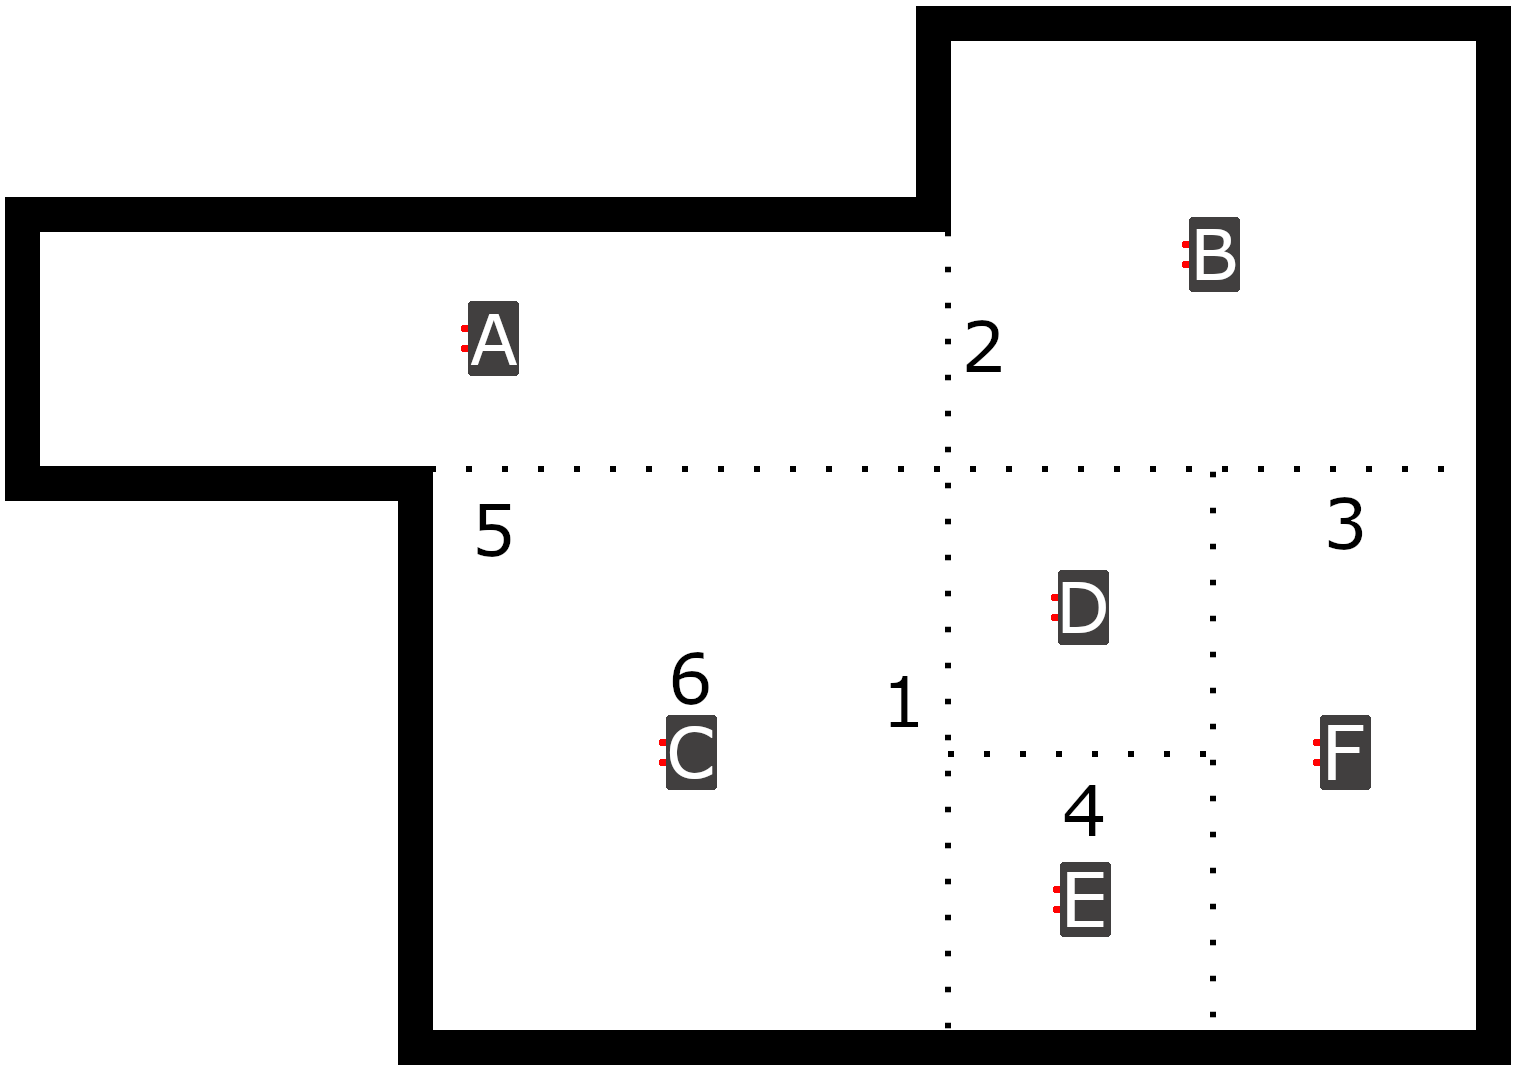
\includegraphics[width=\linewidth]{sble_1_3_floor}
\end{minipage}

\paragraph{Resultaat}
\begin{minipage}{0.55\textwidth}
De resultaten van deze test zijn zichtbaar in bijgevoegde tabel. We zien dat van de 6 beacons er 3 goed en 3 slecht zijn toegewezen. Echter zijn de 3 slecht toegewezen beacons (1, 3 en 5) de beacons die dichter lagen bij de toegewezen locatie gateway dan bij de theoretisch correcte locatie gateway. De andere 3 beacons (2, 4 en 6) zijn wel correct toegewezen. 
\end{minipage}
\hfill
\begin{minipage}{0.42\textwidth}
	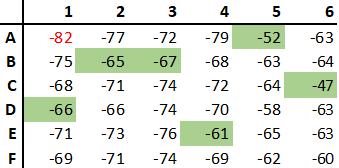
\includegraphics[width=\linewidth]{sble_1_3_results}
\end{minipage}

\paragraph{Testconclusie}
Deze test bevestigd het vermoeden dat deze lokalisatie strategie het slechter zal doen bij locaties van verschillende groottes, door de basering op RSSI en afstand, en dit zeker in een open ruimte waar deze afstand de enige bepalende factor voor de RSSI is (uiteraard buiten de onzekerheden vastgesteld tijdens het BLE vooronderzoek). Een mogelijke remedie hiervoor is ee RSSI filter te plaatsen op gateways voor kleinere locaties, zodat het gebied dat ze (stelen) van aanpalende grotere ruimtes verminderd. Echter omdat het bereik nog steeds (theoretisch) een cirkel blijft zullen vreemde verschijnsels bij locatieovergangen onvermijdelijk blijven.

\subsubsection{Test 3: 5 realistische locaties}
\begin{minipage}{0.55\textwidth}
Deze derde een laatste test vergroot het concept vn vorige test en voegt muren toe zodat de opstelling realistischer wordt. Deze opstelling bestaat uit 5 locaties, ondergebracht in 5 ruimtes van verschillende groottes, gescheiden door muren. Hier is dus afstand niet meer de enige bepalende factor voor de RSSI, maar ook tussenliggende muren. Wat in theorie een groter verschil zou moeten geven, en het grootteverschil tussen locaties wat zou kunnen compenseren. Dit experiment zal ook 2x worden uitgevoerd, 1x met tussenliggende deuren gesloten, en 1x open, om ook het mogelijke effect van deuren vast te stellen.
\end{minipage}
\hfill
\begin{minipage}{0.42\textwidth}
	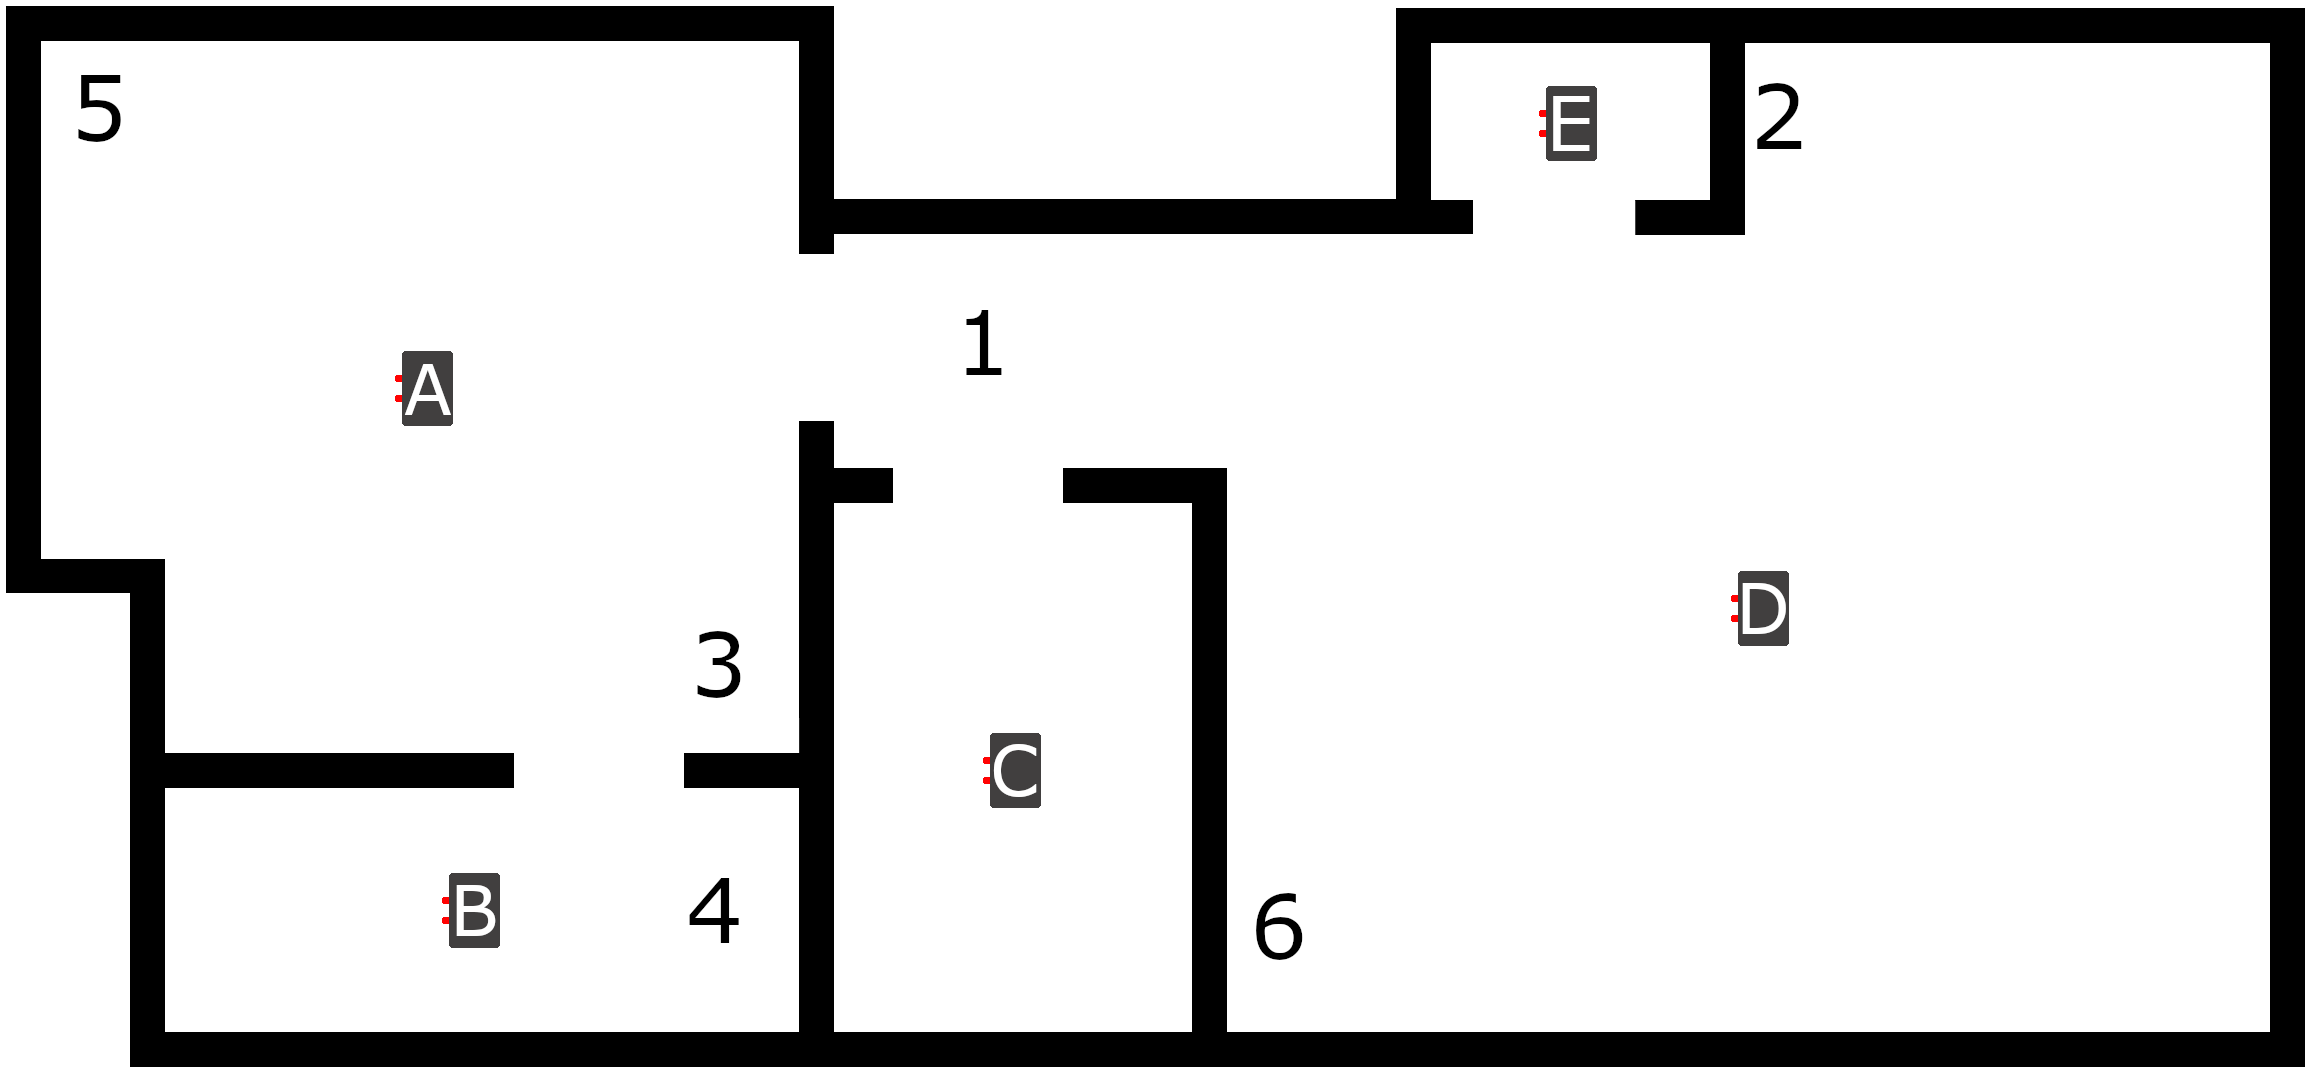
\includegraphics[width=\linewidth]{sble_1_4_floor}
\end{minipage}

\paragraph{a) Deuren gesloten}
\begin{minipage}{0.55\textwidth}
Uit de resultaten is af te leiden dat dit principe zeer goed werkt, met een perfecte lokalisatie. Dit is geen verassing voor da duidelijke, safe beacons (4 en 5). Maar de andere 4 beacons liggen stuk voor stuk in een locatie maar dichter bij een andere gateway (weliswaar met een muur tussen). Met in het bijzonder beacon 2, welke op ong 50cm (+muur) ligt van gateway E, en op 250cm van gateway D, maar nog steeds correct bij locatie D wordt gecategoriseerd.
\end{minipage}
\hfill
\begin{minipage}{0.42\textwidth}
	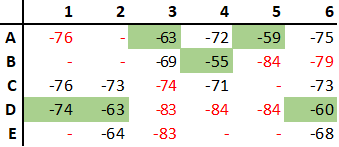
\includegraphics[width=\linewidth]{sble_1_4a_results}
\end{minipage}

\paragraph{b) Deuren open}
\begin{minipage}{0.55\textwidth}
Deze resultaten tonen geen noemenswaardig verschil met de test met gesloten deuren. Alles blijft correct gecategoriseerd, maar ook de waardes verschillen niet veel. Dit is vooral verrassend bij beacon 1, welke met open deur rechtstreeks zichtbaar is voor gateway A, maar toch correct bij gateway D blijft ingedeeld.
\end{minipage}
\hfill
\begin{minipage}{0.42\textwidth}
	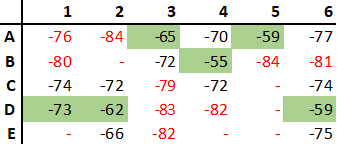
\includegraphics[width=\linewidth]{sble_1_4b_results}
\end{minipage}
\paragraph{Testconclusie}
Deze test toont mooi aan dat de extra isolatie van een muur een positieve invloed heeft op lokalisatie volgens dit principe, en dat een verschil in grote tussen aanpalende ruimtes niet noodzakelijk een groot probleem hoeft te zijn. Uiteraard zal ook het soort muur een invloed hebben op deze resultaten. In de testopstelling worden muren uit cellenbeton gebruikt, maar een dunnere muur uit bv. kalkplaat zal mogelijk een minder isolerend effect hebben. Ook is duidelijk dat een deur weinig impact heeft op de resultaten. Ook dit kan natuurlijk aan het materiaal liggen. Een houten deur zoals in de testopstelling is klaarblijkelijk verwaarloosbaar, maar bv. een nooddeur, speciaal als er metaal in zit, zal een grotere impact hebben.

\subsubsection{Deelconclusie}
Al bij al is dit een zeer acceptabel scenario, het merendeel van de lokalisaties was geslaagd, met uitzondering van fouten aan de locatieovergang in een open ruimte, maar dat is geen verassing na de vaststellingen in het vooronderzoek. Ook bestaat er de mogelijkheid tot toevallige mislokalisaties door hardware effecten, maar dit ligt niet zozeer aan het scenario zelf. De hypothese is bevestigd.

\subsection{Meerdere gateways per locatie}
\subsubsection{Deelhypothese}
Deze opstelling slaagt er in om met een BLE beacon getagde assets correct te lokaliseren.

\subsubsection{Test 1: 2 rechthoekige locaties in reële, open ruimte}
\begin{minipage}{0.55\textwidth}
De testopstelling voor deze eerste test bestaat uit een raster van 6 gateways (analoog aan de opstelling bij het vorige scenario, test 1). De locatiedefinitie is in dit geval in de vakken tussen de gateways, om 2 even grote locaties te creëren. Het idee is dat zichtbaar is aan de meetwaarden in welk vak een beacon ligt, en dus zo een locatie toegewezen krijgt. Meer specifiek aan de laagste som van RSSI's van de gateways in de hoekpunten. 
\end{minipage}
\hfill
\begin{minipage}{0.42\textwidth}
	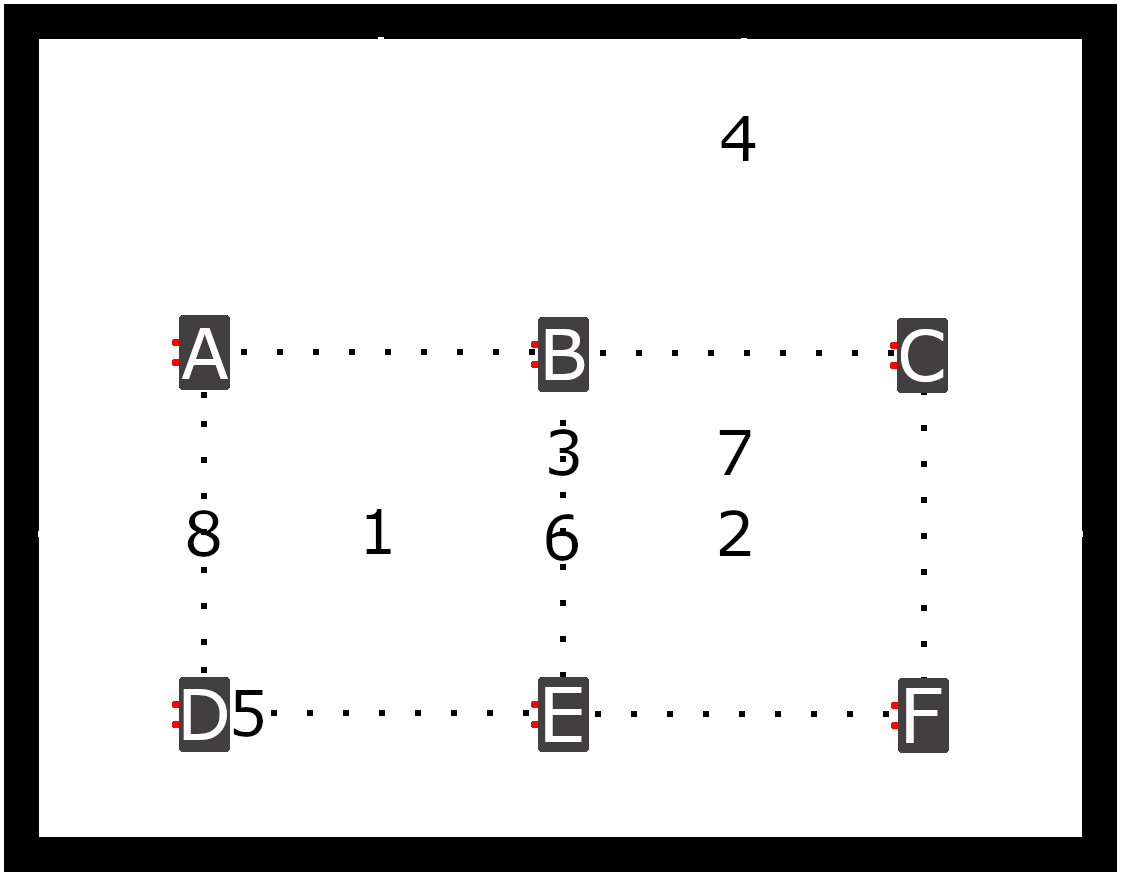
\includegraphics[width=\linewidth]{sble_2_1_floor}
\end{minipage}

\paragraph{Resultaat}
Bijhorende resultaten zijn verrassend goed, met voor elke van de 8 beacons een correcte lokalisatie. Enkele interessante randgevallen zijn beacon 3 en 6, welke op de grens tussen de 2 locaties liggen. Bij beide zijn de cijfers duidelijk voor de rechtse locatie, nochtans zou men verwachten dat deze cijfers dichter bijeen zouden liggen. Verder is er ook beacon 4, welke op geen enkele locatie ligt en is ingedeeld bij de rechtse locatie. Deze indeling is uiteindelijk de correcte, aangezien dit de dichtstbijzijnde locatie betreft en er geen 'geen locatie' mogelijk is in dit experiment. 

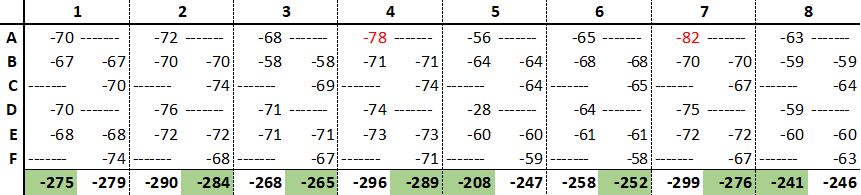
\includegraphics[width=\linewidth]{sble_2_1_results}

\paragraph{Testconclusie}
Deze opstelling heeft in deze eerste test een perfecte lokalisatie gedaan, en is daarmee voorlopig zeer goed. Echter is er het detail van de 'geen locatie' beacons, maar dit is in elk scenario een ding. Hier is dit in theorie oplosbaar aangezien er een bepaalbare bovengrens in som van RSSI's wil de beacon nog tussen de gateways liggen. Deze is ook theoretisch berekenbaar gegeven de afstand tussen de gateways, de FSPL formule en enige meetkundige kennis, maar gezien het vastgestelde verschil tussen theorie en praktijk tijdens het vooronderzoek lijkt dit eerder een maximum dat moet worden gemeten/bepaald.

\subsubsection{Test 2: 2 rechthoekige locaties gescheiden door muur}
\begin{minipage}{0.55\textwidth}
De opstelling voor deze test is analoog an de vorige, het enige verschil is dat er een muur is verschenen tussen de 2 locaties. Dit zal in praktijk ook meer het geval zijn, nl. 2 aanpalende lokalen. Het doel van deze test is om het effect van deze muur op de cijfers te bekijken.
\end{minipage}
\hfill
\begin{minipage}{0.42\textwidth}
	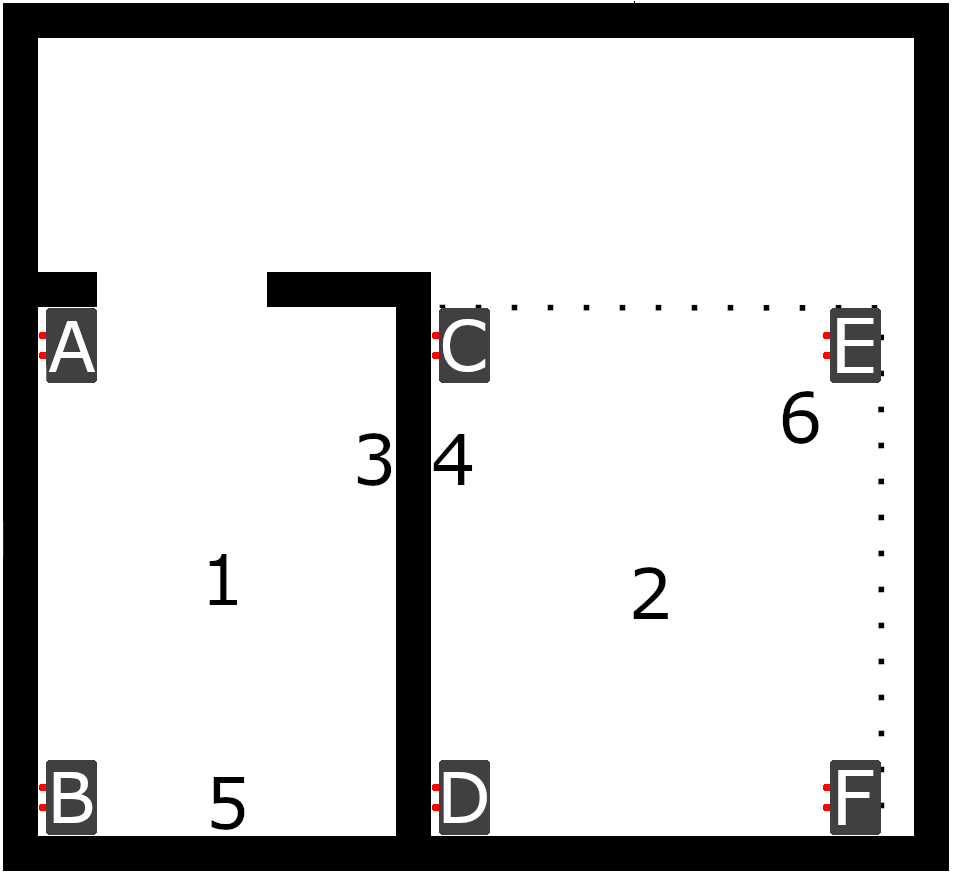
\includegraphics[width=\linewidth]{sble_2_2_floor}
\end{minipage}

\paragraph{Resultaat}
In deze 2e test is dit scenario er ook weer in geslaagd elke beacon correct te lokaliseren. Hier is wel een extra stap bij de verwerking gekomen. Door het toevoegen van de muur wordt niet elke beacon door elke gateway meer opgevangen. Hierdoor verschijnen er rode platte streepjes in de tabel. Het spreekt voor zich dat dit ook meteen diskwalificerend werkt voor de locatie(s) waarvan deze gateway een hoekpunt is aangezien de beacon niet tussen deze gateways zal liggen als er 1 van deze gateways de beacon niet eens ziet.
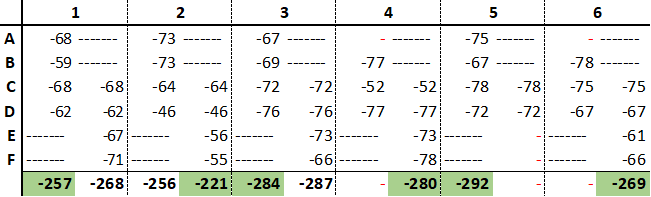
\includegraphics[width=\linewidth]{sble_2_2_results}

\paragraph{Testconclusie}
Op het eerste zicht lijkt deze test volledig geslaagd, het toevoegen van een muur zorgt er niet voor dat dit scenario slechter presteert. Echter is er wel een belangrijk detail dat aangehaald moet worden. Als de cijfers beter onderzocht worden blijkt het volgende: bij elke beacon is de gateway die hem met de hoogste RSSI waarneemt een gateway die in dezelfde ruimte ligt als de beacon. Met andere woorden dezelfde uitkomst kan bekomen worden met 1 gateway per ruimte, en zo wordt de opstelling vereenvoudigd tot het vorige scenario, waarvoor minder gateways nodig zijn.

\subsubsection{Deelconclusie}
Dit scenario blijkt zeer effectief te zijn en heeft alle geteste beacons perfect gelokaliseerd. Echter blijkt wel dat deze opstelling geen voordelen heeft over de vorige (1 gateway / locatie) als een locatie 1 ommuurde ruimte is, maar wel meer hardware vereist. Hiervoor is het dus niet geschikt. Voor lokalisatie in een open ruimte echter, lijkt ze beter te werken, voor een hogere hardware kost. De deelhypothese is bevestigd.

\subsection{Gateways in rasteropstelling}
\subsubsection{Deelhypothese}
Deze opstelling slaagt er in om met een BLE beacon getagde assets een positie te geven binnen het raster zodat het eenduidig met een locatie kan worden gelinkt.

\subsubsection{Test 1: Raster in open, reële ruimte}
\begin{minipage}{0.55\textwidth}
De opstelling voor deze test is idem aan het vorige scenario, test 1. Aangezien bij die test ook beacons in een raster gemeten zijn, kon de data uit die test hier hergebruikt worden en worden verwerkt met trilateratie. Voordat trilateratie kan toegepast worden, moet er eerst een omzetting gebeuren tussen de RSSI waarde en de afstand. Dit kan door de FSPL formule te gebruiken (weliswaar omgekeerd). Aangezien bij de verwerking van de resultaten bleek dat dit niet geheel correct was is nog een offset in dBm toegevoegd, verschillend per soort beacon. Dit om het, bij het vooronderzoek vastgelegde fenomeen dat beacons, hoewel ze de zelfde instellingen hebben, niet allen een even sterk signaal sturen. Bij de verwerking is een waarde gebruikt van -16 dB voor de gebruikte H5 beacons, en -10 dB voor de M2 beacons. Deze waardes zijn experimenteel vastgelegd, en vloeien voort uit de data van de afstandstest bij het vooronderzoek, waar de offset van de trendlijn tegenover de theoretische curve is gebruikt.
\end{minipage}
\hfill
\begin{minipage}{0.42\textwidth}
	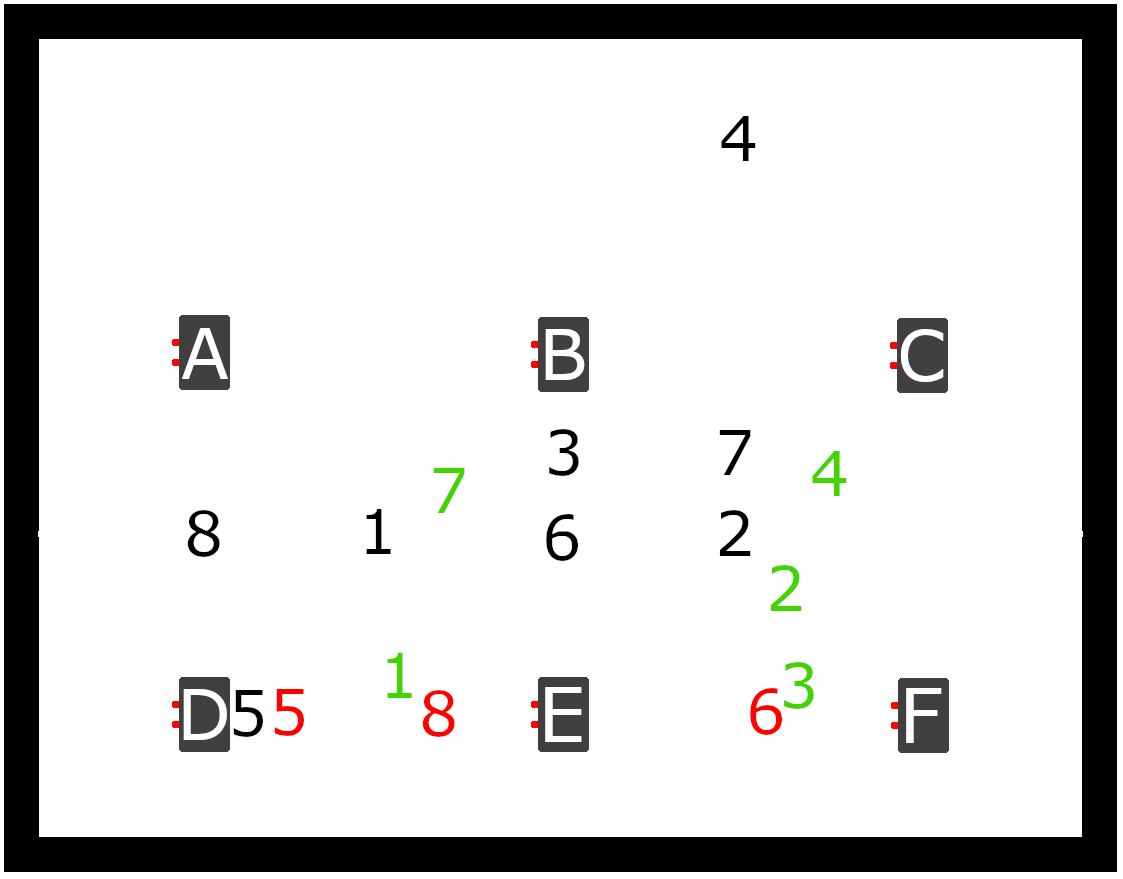
\includegraphics[width=\linewidth]{sble_3_1_floor}
\end{minipage}

De resultaten van de trilateratie worden geplot op bovenstaand grondplan. De zwarte cijfers zijn de effectieve locaties van de beacons, de gekleurde zijn de berekende locaties a.d.h.v. de resultaten en trilateratie, met de groene een geslaagde trilateratie, en een rode een mislukte. Een mislukte wilt zeggen dat trilateratie niet mogelijk is door te korte afstanden (bv. de afstand tussen beacon 6 en gateway E en F bedraagt resp. 0.87m en 0.62m, dus opgeteld 1.49m. Dit is onmogelijk aangezien de afstand tussen deze beacons 2m bedraagt). Bij een situatie zoals dit is de beacon geplaatst tussen de 2 gateways.

\paragraph{Resultaat}
Om het resultaat te berekenen zijn de 2 gateways met de beste RSSI gebruikt. Meteen is zichtbaar dat het resultaat vrij catastrofaal is en dat de uitkomst van de trilateratie de beacons precies random plaatst. Beacon 5 komt in de buurt, maar deze lag fysiek aan gateway 5, waardoor zijn RSSI zeer hoog was (-28 dBm), hierdoor werd deze door de noodoplossing van het algoritme toch ietwat in de buurt geplaatst maar dit is een unicum. Verder is enkel beacon 2 relatief ok geplaatst.

\paragraph{Testconclusie}
Het is duidelijk dat trilateratie op basis van RSSI zeer onnauwkeurig is. Dit ligt vooral aan het onnauwkeurig omzetten van RSSI waardes in afstanden door de grote onzekerheden op RSSI waardes. Deze eerste test belooft zeker niet veel goeds voor dit concept.

\subsubsection{Test 2: Raster in verspreid over gebouw met muren}
\begin{minipage}{0.55\textwidth}
In deze 2e test is het raster vergroot, van 2m maar 3.5m tussen gateways. Ook is het raster verspreid over een gebouw, met muren tussen.
De methodieken voor berekening en de kleurcodes voor het visualiseren van de resultaten zijn gelijk gebleven aan vorige test.
\end{minipage}
\hfill
\begin{minipage}{0.42\textwidth}
	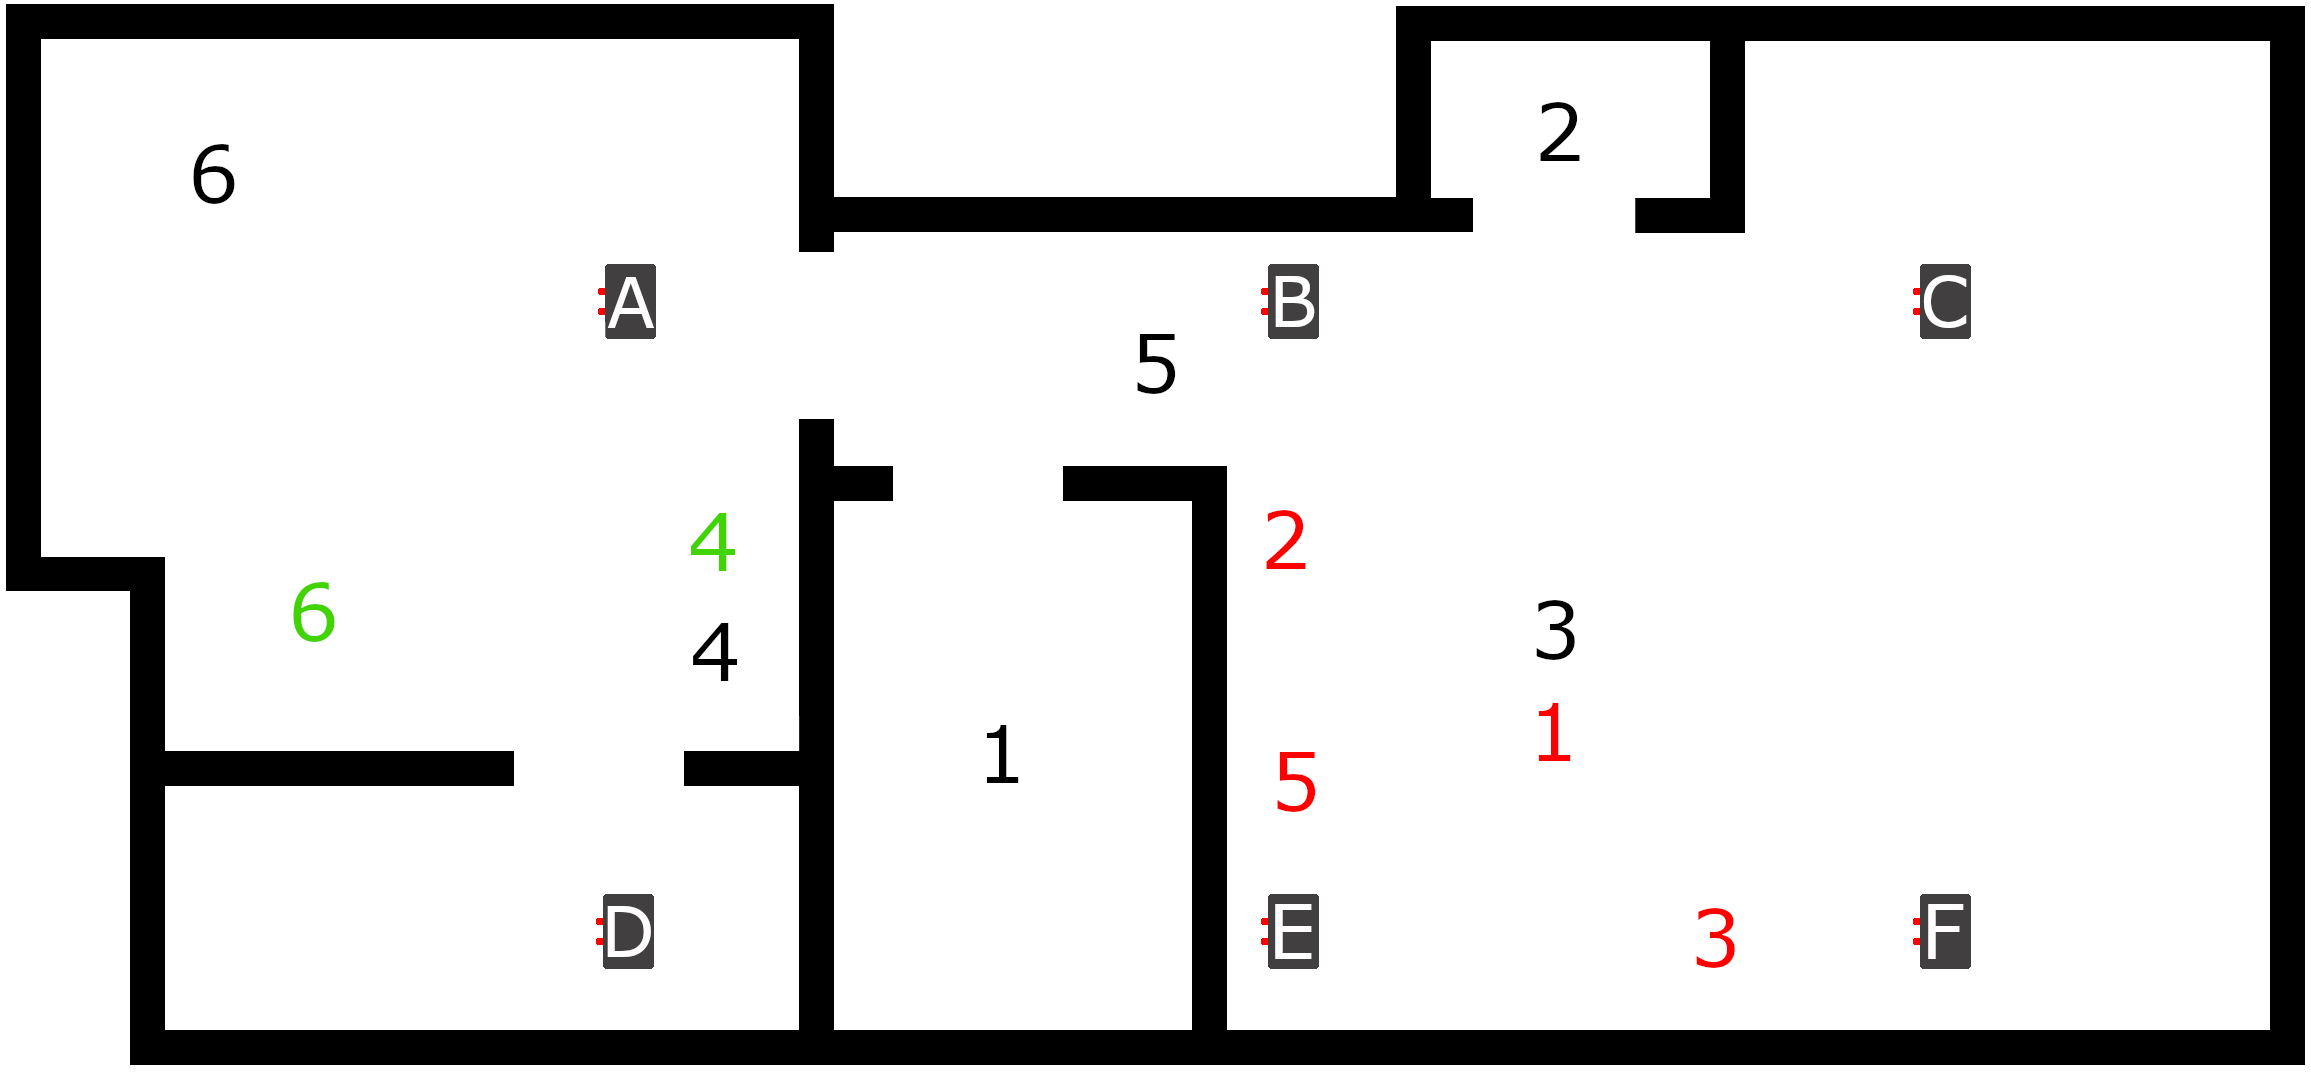
\includegraphics[width=\linewidth]{sble_3_2_floor}
\end{minipage}

\paragraph{Resultaat}
\begin{minipage}{0.55\textwidth}
Na deze test zijn er slechts 2 beacons die met succes kunnen getrilatereerd worden zonder de noodoplossing te gebruiken (groen). Deze 2 beacons (4 en 6) zijn ook enkel opgemerkt door de 2 gateways waar ze tussen liggen. De 4 andere beacons zijn zeer slecht geplaatst in vergelijking met hun effectieve positie.
\end{minipage}
\hfill
\begin{minipage}{0.42\textwidth}
	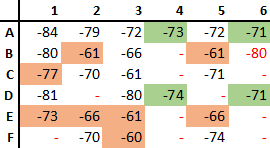
\includegraphics[width=\linewidth]{sble_3_2_results}
\end{minipage}

\paragraph{Testconclusie}
Deze grotere test heeft weer aangetoond wat na vorige test al duidelijk was, trilateratie op basis van RSSI is onnauwkeurig. En het toevoegen van muren, waardoor niet elke geteway meer elke beacon ziet, heeft de nauwkeurigheid enkel verslecht.

\subsubsection{Deelconclusie}
Na deze 2 tests kan duidelijk worden besloten dat dit scenario niet haalbaar is met de gebruikte BLE hardware. In het principe zit potentieel, maar enkel als er een goeie, precieze conversie kan worden gemaakt tussen RSSI waardes en afstanden. De deelhypothese is hierbij dus ontkracht.

\subsection{1 beacon per locatie, midden van locatie}
%TODO

\subsection{1 beacon per locatie, aan deur}
%TODO

\subsection{Meerdere locatiebeacons per locatie}
%TODO

\subsection{Beacons in rasteropstelling}
\subsubsection{Deelconclusie}
Na de zeer slechte testresultaten van de statische versie van dit scenario, en omdat dit scenario zich qua principe berust op dubbele trilateratie, waardoor de extreme onnauwkeurigheden bij enkele trilateratie enkel maar extremer zullen worden, is besloten dit scenario in te delen in dezelfde categorie.

\subsection{Beacons op intervallen in de gang}
%TODO
